\documentclass[12pt,french]{report}
\usepackage[utf8]{inputenc}
\setcounter{secnumdepth}{3}
\setcounter{tocdepth}{3}
\usepackage{textcomp}
\usepackage{graphicx}
\usepackage{nomencl}
% the following is useful when we have the old nomencl.sty package
\providecommand{\printnomenclature}{\printglossary}
\providecommand{\makenomenclature}{\makeglossary}
\makenomenclature

\makeatletter

%%%%%%%%%%%%%%%%%%%%%%%%%%%%%% LyX specific LaTeX commands.
\DeclareFontEncoding{LGR}{}{}
\DeclareRobustCommand{\greektext}{%
  \fontencoding{LGR}\selectfont\def\encodingdefault{LGR}}
\DeclareRobustCommand{\textgreek}[1]{\leavevmode{\greektext #1}}
\ProvideTextCommand{\~}{LGR}[1]{\char126#1}

%% Special footnote code from the package 'stblftnt.sty'
%% Author: Robin Fairbairns -- Last revised Dec 13 1996
\let\SF@@footnote\footnote
\def\footnote{\ifx\protect\@typeset@protect
    \expandafter\SF@@footnote
  \else
    \expandafter\SF@gobble@opt
  \fi
}
\expandafter\def\csname SF@gobble@opt \endcsname{\@ifnextchar[%]
  \SF@gobble@twobracket
  \@gobble
}
\edef\SF@gobble@opt{\noexpand\protect
  \expandafter\noexpand\csname SF@gobble@opt \endcsname}
\def\SF@gobble@twobracket[#1]#2{}
%% A simple dot to overcome graphicx limitations
\newcommand{\lyxdot}{.}


%%%%%%%%%%%%%%%%%%%%%%%%%%%%%% Textclass specific LaTeX commands.
\newenvironment{lyxlist}[1]
{\begin{list}{}
{\settowidth{\labelwidth}{#1}
 \setlength{\leftmargin}{\labelwidth}
 \addtolength{\leftmargin}{\labelsep}
 \renewcommand{\makelabel}[1]{##1\hfil}}}
{\end{list}}

\@ifundefined{date}{}{\date{}}
\makeatother

\usepackage{babel}
\makeatletter
\addto\extrasfrench{%
   \providecommand{\og}{\leavevmode\flqq~}%
   \providecommand{\fg}{\ifdim\lastskip>\z@\unskip\fi~\frqq}%
}

\makeatother
\begin{document}

\title{{*}}

\maketitle
\begin{titlepage}
 \begin{center}
    \Large
     Zürcher Hochschule der Künste\\
 	en collaboration avec l' Interkantonale Hochschule für Heilpädagogik \\
	 MAS Klinische Musiktherapie Master of Advanced Studies en musicothérapie clinique\\
  \vfill
  { \LARGE
\emph{Le test d'écoute en musicothérapie }\\ \bigskip
	 }
 \vfill
 \end{center}
MéMOIRE  POUR L'OBTENTION  du titre de
Musicothérapeute
MASTER OF ADVANCED STUDIES KLINISCHE MUSIKTHERAPIE présenté par VALéRIE GAILLARD

Directeur de mémoire : Anne Bolli

 {\large

	 Valérie Gaillard    \hfill Genève\\
	 \rule{0mm}{1pt} \hfill printemps 2018}

\end{titlepage}
\begin{abstract}
Se visualiser, se voir, se découvrir à travers le reflet de son écoute.
Situer des sons dans l'espace pour se positionner soi-même. Se situer
dans l'espace sonore.

Ecouter et s'écouter.

Un test d'écoute pourrait avoir un sens pour le patient, qui visualiserait
son écoute. Le fait de tester des sons précis permettrait de déclencher
un travail, un début de cheminement intérieur.

Le test deviendrait-il aussi un outil intéressant pour le thérapeute
qui saisirait le patient de manière différente ? Se situer dans l'espace
sonore implique tout son corps, demande un effort, une prise de conscience,
une prise de distance avec soi-même et pourrait être considéré comme
un point de départ dans un traitement en musicothérapie. 

Cette étude a pour objet de faire l'hypothèse d'une possible visualisation
de la modification, de la transformation de l'écoute d'une personne
lorsque cette personne suit un traitement en musicothérapie. Nous
citerons brièvement les travaux les plus récents prouvant l'impact
de la musique sur le cerveau grâce à l'IRMfct mais nous nous étendrons
pas outre-mesure sur ce sujet. Nous nous limiterons intentionnellement
à ne faire qu' une sorte de ``photographie'' d'une écoute en début
de traitement en musicothérapie et à la comparer avec une seconde,
faite à la fin de celui-ci.

La musicothérapie fait partie de ces thérapies dites subtiles. Elle
est très difficilement quantifiable comme le fait par exemple, la
psychologie cognitivo-comportementaliste, avec des tests. Il n'y a
jamais, à proprement parlé, d'avant et d'après mais il y a transformation.
Et les transformations échappent toujours aux quantifications. Peut-être
ici pourrons-nous apporter un outil plus objectif par un test particulier
d'écoute : la démonstration d'un travail d'écoute, d'une perception
différente, d'une sensibilité nouvelle du patient. Apprendre à écouter,
c'est un travail et des résultats pourraient être visibles.

Mots-clés : la musicothérapie- Tomatis-l'écoute-l'oreille-le test-la
perception- la transformation-l'apprentissage de l'écoute
\end{abstract}
\tableofcontents{}

\chapter{Introduction et Hypothèse : }
\begin{quotation}
``\emph{ Par le Son, le Silence du Non-Être vient à l'Être. Je suis
la musique que je fais ou écoute. La musique a la capacité d'harmoniser
les composantes d'une entité psychophysique pour qu'il soit ``bien
dans sa peau'' et ``bien dans son âme''. Jacques Viret }\footnote{\emph{B. A-BA de la musicothérapie,(2007)} éd.Pardès}
\end{quotation}
J'exerce le métier de musicienne professionnelle depuis de nombreuses
années. Par la suite, je suis aussi devenue musicothérapeute, formée
également en tant que consultante à la méthode Tomatis, études suscitées
par mon intérêt croissant au sujet du développement de la personne
à travers l'outil que nous offre la musique : le son.

Dans ma pratique, les deux formations ont successivement pris plus
ou moins d'importance, selon les périodes de travail en clinique psychiatrique,
en réhabilitation à la SUVA, ou selon mon travail dans mon cabinet
privé. En clinique, ce sera exclusivement la musicothérapie. En cabinet
privé, j'aurai la liberté de choix dans l'utilisation des méthodes.
C'est ainsi que, peu à peu, à travers chaque cas particulier du patient,
j'ai vu mes techniques d'approche et de soin se modifier, évoluer,
pour parfois, aller se fusionner. Dans ce cheminement, de nombreuses
interrogations se sont imposées et continuent de m'interpeller.

Ce qui m'a animée? C'est de creuser et d'approfondir mes recherches.
Cette démarche me semble originale, quoique Jacques Bonhomme, spécialiste de la voix, a aussi utilisé ce test dans son travail. Mais le domaine psychiatrique dans lequel je fais cette  recherche est différent.
 Pourrai-je être plus précise dans mes
observations? Pourrai-je clarifier ma manière de travailler qui est celle de mixer les deux méthodes ?

\textbf{Hypothèse}:\\ 
\begin{enumerate}
	\item \textit{Un test d'écoute comme outil musicothérapeutique :}
\end{enumerate}

En partant de l'utilisation d'un test d'écoute spécifique employé
dans la thérapie  Tomatis, l'hypothèse suivante s'est imposée à moi : ce test d'écoute
pourrait-il servir aux musicothérapeutes? Y aurait-il moyen de donner
un champ de \emph{vision de l'écoute }du patient suivi exclusivement
en musicothérapie ? Nous avons ici exclu les traitements des musiques appliquées dans la méthode Tomatis, car nous devions nous limiter à un seul lieu et contexte- une clinique psychiatrique- où l'application de cette méthode n'a pas été possible pour ce travail.  Il y a eu aussi une limitation dans le temps, liée à mon 10%. Ainsi les changements et les fluctuations d'écoute relevées par les tests Il serait s'agit d'une comparaison des différentes utilisations du son.

Ce domaine est très vaste et la façon d'utiliser les sons et de les
traiter l'est aussi. L'objet de cette étude est de faire un constat
qui pourrait donner matière à réflexion tout en ne confrontant pas
les différentes techniques employées - qui pourraient avoir plus ou
moins d'impact quant à l'évolution du travail du patient.

Ma recherche est celle-ci : est-il pertinent d'utiliser ce test d'écoute
Tomatis en musicothérapie? Un support graphique, visible, presque
``palpable'', avec des critères d' interprétations, pourrait-il
donner une ``dessin'', une image utile, utilisable, tangible ? Permettrait-il
de visualiser plus objectivement les changements, la transformation
de l'écoute du patient et la démonstration de ce travail? un travail
qui mettrait à jour une perception différente, une sensibilité nouvelle?

Ne serait-ce pas là une démonstration tangible du travail de la musicothérapie
? La musique est aérienne. En comparaison avec l'art-thérapie, qui
peut nous apporter des supports graphiques, concrets du travail psychique
d'un patient, la musicothérapie pourrait être, d'une certaine façon,
visuellement aussi plus claire, et ce, en priorité dans l'esprit du
patient pour lui-même. 

Comme l'exprime à juste titre André Malraux : ``\emph{Le monde de
l'art n'est pas celui de l'immortalité , c'est celui de la métamorphose.''}
De même, la musique est un art produit par l'homme et qui a un impact
sur lui-même. Les deux interagissent, s'interpénètrent et s'auto-transforment
au cours des siècles. Ce que nous pourrons constater lors de l'aboutissement
d'une thérapie n'est pas de trouver une autre personne mais une transformation
de la perception de celle-ci par rapport au monde qui l'entoure. Selon
ce que nous vivons, nous nous transformons mais continuons à être
soi. Nous continuons à ``être soi'' mais autrement. Nous ne perdons
pas notre identité.


\paragraph{{\tiny{\normalsize  Dans la première partie, j'aborderai l'aspect théorique : le test}}
d'écoute, les différents sortes de tests d'écoute en musicothérapie,(
Verdeau-Paillès, Auriol). Ensuite, nous expliquerons la méthode Tomatis
et puis, beaucoup plus en détail, son test d'écoute. }

\paragraph{En deuxième partie : ce sera l'aspect clinique : les résultats ,
les études de cas, les tests faits en clinique avec deux groupes de
comparaison.}

\paragraph{Et finalement, vérification de l'hypothèse, conclusions et interrogations.}

\chapter{L'écoute :}

\section{Ecouter ou entendre : une différence}

Nous commencerons par la définition du verbe ``entendre'' et du
verbe ``écouter'', faite par le dictionnaire Hachette, édition 2012.
Ceci nous paraît opportun par le fait qu'il y a souvent confusion,
mélange et utilisation des deux termes de manière indistincte : 
\begin{enumerate}
\item \emph{Entendre }: percevoir des sons, saisir par l'ouïe
\item \emph{Ecouter} : a).prêter l'oreille pour entendre b).prêter attention
à l'avis de quelqu'un, suivre un avis.c). fig suivre une impulsion,
une inspiration.
\end{enumerate}
La première action est en soi, passive, involontaire, non sélective. 

Tandis que la deuxième est active, implique la volonté, permet une
forme de décodage : Il s'agit d'un acte, d'une action, d'une capacité.\emph{
}Lorsque nous lisons attentivement, nous faisons abstraction des bruits
environnants, nous les entendons parfaitement mais nous n'y prêtons
pas attention. Nous parvenons à couper les sons parasites pour nous
concentrer que sur les sons pertinents.

\emph{Entendre} est une attitude passive par rapport au monde sonore
qui nous entoure. Nous recevons les sons sans les interpréter et cela
ne demande aucun effort.

Tandis qu'\emph{écouter} est une opération de tout autre nature puisqu'elle
suppose une participation active dans le choix du message ou dans
la sélection d'une voix.

Bernard Auriol, cité plus bas (note 6) ouvre son livre ``La Clef
des sons'' par cet en-tête . ``L'écoute est une action'' et par
ces deux phrases : ``Entendre suppose un son (physique), une oreille
pour le capter, un système nerveux pour le recevoir. Ecouter est un
processus actif supposant préférences et répulsions pour tel son ou
telle séquence sonore.''

Entendre et écouter sont donc des processus bien différents, \footnote{Extrait de l'entretien réalisé par Bernard Auriol avec Alfred Tomatis,1973 }``deux
fonctions essentiellement distinctes bien qu'évoluant apparemment
sur des terrains identiques.'' Tomatis met l'accent sur `` l'élément
conscient, facteur essentiel sur lequel repose toute la différence
entre ces deux activités''.

Pour exemple concret, nous savons qu' un enfant autiste peut entendre
parfaitement bien, souffrant même d'hypersensibilité aux sons mais
qui malgré tout n'écoute pas.\emph{ }

\emph{``Ecouter} se base certes sur une stimulation prenant sa source
à I'extérieur mais \emph{devant êre intérieurement, intentionnellement
recherché}e.'' 

Tomatis fait également un parallèle très clair avec ``voir et vouloir
voir''. Ce sont deux mécanismes totalement différents, le second
utilisant le premier. \emph{``Vouloir voir, c'est viser. }Il en est
de même pour entendre et écouter.\emph{ L\textquoteright écoute résulte
du vouloir entendre }et est l\textquoteright équivalent de la visée.\emph{
``}

Et puis, lorsque l'on considère au sens figuré c) la définition d'écouter
: suivre une impulsion, une inspiration, ne correspondrait-elle pas
au but ultime de la démarche d'ouverture imbriquée dans la notion
même de l'écoute ? Ne serait-ce pas aussi, dans cette démarche, celle
de s'ouvrir à une autre forme d'écoute, donnée par l'inspiration ou
induite par une impulsion? 

D'autre part, il est fort intéressant de se poser la question de l'objectivité
ou de la subjectivité de notre écoute. Nous avons tous anatomiquement
parlant, à peu de choses près, la même oreille. Logiquement, nous
devrions entendre et écouter la même chose lors d'une même information
diffusée. Pourtant, cela ne semble pas se passer ainsi. Chacun n'entend
pas de la même manière les mêmes informations, en somme, tout un chacun
entend ce qu'il veut bien entendre. Nous approfondirons plus loin
le chapitre lié à la méthode Tomatis et du rôle important que semble
jouer notre cerveau à notre écoute. 

Ainsi l'écoute est une fonction exceptionnelle, innée en l'homme mais
qui semble pas si simple car elle demeure souvent enfouie et occultée.

\section{Le test d'écoute :}

Qu'est-ce qu'un test d'écoute ?

Dans le milieu médical, il s'agit d'un test, nommé audiogramme qui
sert à mesurer les seuils d'audition des sujets, grâce à l'audiomètre,
appareil français qui avait été mis au point en 1933. Les Américains
ont repris ces travaux pendant la dernière guerre pour pouvoir dépister
les dommages subis par ceux qui conduisaient des engins bruyants comme
des avions.

C'est une épreuve d'ordre physiologique, voire anatomique.\emph{ }Elle
est pour \marginpar{otologie : branche de la médecine qui étudie l'oreille et ses maladies}l\textquoteright otologiste
un examen fondamental à partir duquel se dessinent les données \footnote{étiologie : étude des causes d'une maladie}étiologiques
d'un trouble de la fonction auditive. D'elle dépend, en outre, le
pronostic qui va orienter le mode de thérapie médicale ou chirurgicale,
ou bien encore prothétique, voire rééducative. 

Existe-t-il d'autres formes de tests d'écoute?

Dans nos recherches sur internet ( décembre 2016) , il nous est proposé
de tests d'écoute en majorité présentés sous une forme verbale tels
que par exemple celui que Roger Lanteri ou de Bruno Daigle, qui mettent
l'accent sur la communication ou une capacité d'empathie. Ils sont
donc de nature purement psychologique. Cela va de pair avec la définition
même du verbe écouter citée plus haut. Mais ces tests sont des tests
d'écoute sans élément sonore à déceler. Est.-ce que l'élément sonore
apporterait davantage d'informations sur le patient ?Pour quelles
raisons la matière sonore ne pourrait-elle pas directement servir
d'élément d'évaluation du sujet pour les musicothérapeutes ? 

Nous avons étendu nos recherches de tests d'écoute qui seraient actuellement
utilisés dans cet optique.

Avec la psychanalyste Jacqueline Verdeau-Paillès qui a étudié et intégré
la psychanalyse avec le son, le sonore est introduit sous forme réceptive,
avec un test d'audition d'oeuvres. Elle est définie comme une technique
complémentaire de musicothérapie qui permet d\textquoteright entreprendre
une relation analytique. 
\begin{itemize}
\item Test de Verdeau-Paillès :\footnote{\emph{``Le bilan psycho-musical et la personnalité}''Dr.Jacqueline
Verdeau-Paillès.Ed.Fuzeau} Celui-ci permet d'étudier la place qu'occupent la musique et le sonore
dans la vie du patient : le type de réceptivité à la musique et les
possibilités de communication à l'aide de la musique et des sons.
C'est une démarche en trois volets qui développe un entretien, un
test d'audition d'oeuvres et un texte actif pour répondre à trois
objectifs : une meilleure connaissance de soi, l'aide à l'établissement
d'un projet thérapeutique et le travail psychopédagogique. Les recherches
de Benenzon\footnote{Rolando Omar Benenzon,'' \emph{La musicothérapie, la part oubliée
de la personnalité''}} ont été reprises par Verdeau-Paillès pour l'élaboration de ce test.
En un peu plus de détails, voici ce qu'il en est :
\end{itemize}
\begin{quote}
``La technique du montage en U : Comparable aux effets de la sophrologie
et de la relaxation en général, cette technique est surtout utilisée
dans le traitement de la douleur, de l\textquoteright anxiété et de
la dépression. Il est généralement recommandé de procéder à des séances
de durée variable de 20 à 45 minutes et décomposées en plusieurs phases
de 5 à 6 morceaux. Ces morceaux de 3 à 4 minutes chacun, fondus et
enchaînés, amènent progressivement le patient à la détente. L\textquoteright implication
et la coopération du patient sont primordiales. La détente, le détournement
de l\textquoteright attention, la relaxation profonde, et la qualité
de la relation patient-soignant sont des facteurs certains d\textquoteright amélioration.(...).\footnote{(Source : ASSOCIATION AMARC, Association de musicothérapie, recherches
cliniques et applications).}''
\end{quote}
Cette technique analytique, de type individuel, est considéré, selon
cet article, comme complémentaire à la musicothérapie par le pouvoir
même de la musique, déclencheuse d' émotions. Elle est de type individuel
dans le sens qu'elle se base sur un entretien-questionnaire à la première
séance. Lors de l'audition des musiques choisies par le thérapeute
et/ou par le patient, le patient va en verbaliser le vécu et le musicothérapeute
va recevoir et analyser ce qui en émerge. On peut considérer qu'il
s'agit d'une relation tripolaire patient-thérapeute-musique. Elle
favorise''\emph{ l\textquoteright expression et le développement
de la pensée}''et (...) va ``permettre la \emph{prise de conscience
des processus pathologiques développés.'' }

De même avec Fern Nevjinsky, le diagnostic se fera avec des morceaux
de musique et ce, particulièrement en association libre : 
\begin{itemize}
\item Le test de Rorschach(visuel) associé au test musical, de Fern Jevjinsky:
\footnote{``\emph{Adolescence, musique, Rorschach}'' de Fern Nevjinsky, publication
de l'Université de Rouen n\textdegree 215. } La consigne évolue de l'identification de sons à l'association libre
car l'auteur remarque que (...) ``la portée diagnostique du test
fait avec des sons purs, en se limitant à l'identification, est insuffisante
; mais, si la consigne est libre -dire ce que le son signifie- toutes
les perceptions erronnées sont le point de départ d'une expression
fantasmatique en relation avec le passé du sujet, ses souvenirs. En
définitive, cette technique nous permet de nous interroger sur la
valeur priviligiée du son comme éveil des affects liés à des conflits
qui n'apparaissent pas dans l'entretien ou dans les tests visuels.(...
)A un niveau psychanalytique, par le biais de la régression, elle
peut amener le sujet à abandonner une partie de sa vigilance défensive.'' 
\end{itemize}
Cette technique est donc un ``plus'', un élément universel et non
anxiogène, utilisée en test. Fern Nevjinsky utilise ainsi le test
musical en complémentarité de celui de Rorschach.

En définitive, nous revenons donc, avec d'autres façons d'intervenir,
à ce qui a été déjà formulé plus haut dans la technique de Verdeau-Paillès,
à savoir, la musique est un outil déclencheur des expressions et provoque
l'éveil des affects avec leur verbalisation.

Bernard Auriol\footnote{Médecin psychiatre, psychothérapeute, né en 1938, a écrit plusieurs
ouvrages, dont : \emph{Le son au subjectif présent}, Ed. du Non Verbal
(AMBx), 1996, ISBN 978-2906274198\emph{ La clef des sons} {[}archive{]},
2e édition. \emph{Éléments de psychosonique,} Erès, coll. « Études
sociales », 1996, ISBN 978-2865861798, traduction en russe. \emph{Méditation
et psychothérapie} {[}archive{]}, Jean-Marc Mantel, Brigitte Kashtan,
Jacques Castermane, Bernard Auriol, Albin Michel, coll. « Espaces
libres », 2006, ISBN 978-2226149244\emph{ méthode TOMATIS :} }a étendu ses recherches sur le son, la psychosonie, tout en s'inspirant
des travaux d'Alfred Tomatis, avec lequel il s'est également formé.
\begin{itemize}
\item Le terme psychosonique a été créé en 1991 par Bernard Auriol pour
désigner la discipline qui cherche à évaluer et décrire les effets
du son sur l'être vivant (spécialement humain) ainsi que les éléments
subjectifs manifestés par l'expression sonore, en particulier la voix.
Il convient de distinguer la psychosonique de la psychoacoustique
qui se situe davantage du côté de la psychophysique que d'une approche
psychodynamique. La psychoacoustique se préoccupe des conditions acoustiques
et neuro-psycho-physiologiques de l'audition, alors que la psychosonique
tente d'étendre le point de vue aux éléments symboliques, psychodynamiques,
inconscients et subjectifs du processus d'écoute. Bernard Auriol a
mis en place un test des chakras.
\end{itemize}
La psychosonique est, selon cette source internet, très proche de
la musicothérapie, avec une acceptation plus large. 
\begin{itemize}
\item Le test d'écoute Tomatis : Ce test est un outil de diagnostic élaboré
par lui-même. Il est aussi psychologique mais basé sur une chaîne
de sons précis et pareils pour chaque patient. Ils doivent être identifiés
par chaque sujet avec un protocole très clair et des consignes précises
. Il semble s'apparenter à un audiogramme dont le but est de déceler
un trouble de l'audition et son origine. Mais ce n'est pas pareil.
La technique de passation du test ne se déroule pas de la même manière
et, de plus en se fondant sur ces résultats, il est possible de savoir
si le patient désire ou non se servir des sons qu'il a à disposition.
C'est en cela que se situe la différence existant entre un audiogramme
et le test Tomatis. Le patient a peut-être la possibilité d'entendre
un large spectre de sons mais ne souhaite pas, pour diverses raisons
( traumatismes, expériences négatives), forcément les écouter. Son
cerveau aura le pouvoir de les assourdir, puis de les faire disparaître
peu à peu de son champ d'écoute. En résumé, par protection, il choisit
de les annihiler alors que l'oreille peut les collecter. Le cerveau
crée ce que l'on appelle des distortions d'écoute. \footnote{Professeur Tomatis \char`\"{}Education et Dyslexie\char`\"{} Editions
ESF Collection \char`\"{}Sciences de l'éducation\char`\"{}.}
\end{itemize}
\begin{quote}
\emph{``Le test d'écoute sait intégrer ces renseignements dans le
cadre d'un processus psychologique qui va permettre de déceler si
le sujet désire ou non se servir des matériaux qu'il a à sa disposition
sur le plan perceptif. (...)Il est avant tout un test psychologique
et} les données psychologiques vont permettre d'établir un\emph{ diagnostic}
et d'orienter un mode d'action.''
\end{quote}
Est-ce que cette théorie tient la route ? est-ce vraiment possible
? N'est-ce pas un peu paradoxal ? on peut entendre des sons que l'on
n'entend pas!ou que l'on n'écoute pas! Nous allons tenter d'en savoir
d'avantage. Notre cerveau comporte encore beaucoup de mystère et le
domaine des neurosciences est un vaste monde à découvrir. 

Il est à relever que cette façon de procéder et d'aborder un test
d'écoute est originale en comparaison avec les différents tests cités
plus haut.

C'est cette forme d'objectivité \footnote{L'objectivité et la subjectivité ne sont pas des notions simples lorsque
l'on parle du son.}dans le test - la mise en évidence des seuils d'écoute- et en même
temps cette possibilité -d'analyser le potentiel d'écoute de chaque
patient- qui nous ont incité à vouloir en savoir davantage et de porter
notre choix dans l'approfondissement de ce sujet. Les réponses des
patients donnent des indices, des renseignements sur eux-même, et
ce de manière involontaire, sans qu'ils puissent les contrôler d'une
quelconque façon ou les influencer intellectuellement. Ces réponses
sont immédiates et résultent d'une adéquation très simple qui est
celle de signaler un son dès qu'ils l'entendent. Ce sont ces éléments
que nous avons rassemblés lors de notre recherche. Nous y reviendrons
en détails dans le chapitre 3 ; mais voyons dans l'immédiat les caractéristiques
du son, données indispensables pour l'analyse d'un test d'écoute.
\begin{quote}
\footnote{``Considérations sur le test d'écoute. Propos recueillis au cours
du IIIème congrès international d'audio-psycho-phonologie ( Anvers
1973) à la suite d'un entretien avec le professeur Tomatis .Dans son
ouvrage \char`\"{}Éducation et Dyslexie\char`\"{}, le Professeur Tomatis
a présenté le test d'écoute comme étant le test le plus important
du bilan Audio-Psycho-Phonologique et comme devant déterminer les
possibilités d\textquoteright écoute du sujet : auto-écoute et écoute
de l'autre.}
\end{quote}

\section{Le son :}

Le son possède plusieurs caractéristiques physiques. Il peut être
défini très précisément par un ensemble d'unités physiques chiffrées
: les décibels et les hertz. 
\begin{itemize}
\item Un décibel est l'unité de mesure de l'intensité du son. Un décibel
est égal à 1/10 de bel ; une augmentation de l'intensité égale à 1
bel équivaut à peu près à un doublement de l'intensité sonore. 
\item Un hertz est une unité de fréquence\footnote{la fréquence est le nombre de vibrations par unité de temps dans un
phénomène périodique} (symbole : Hz). Équivalent à 1 s-1. Fréquence d'un phénomène périodique
dont la période est une seconde. Ses multiples sont, entre autres,
le kilohertz (kHz), le mégahertz (MHz) et le gigahertz (Ghz). Cette
unité vient du savant allemand Heinrich Hertz, pionnier de la radioélectricité.
\end{itemize}
Le son peut être défini de deux manières : 
\begin{itemize}
\item d'une manière objective tout d'abord : c'est le phénomène physique
d'origine mécanique consistant en une variation de pression (très
faible), de vitesse vibratoire ou de densité du fluide, qui se propage
en modifiant progressivement l'état de chaque élément du milieu considéré,
donnant ainsi naissance à une onde acoustique (la propagation des
ronds dans l'eau suite à un ébranlement de la surface donne une bonne
représentation de ce phénomène) ; 
\item d'une manière subjective également : il s'agit de la sensation procurée
par cette onde, qui est reçue par l'oreille, puis transmise au cerveau
et déchiffrée par celui-ci.\index{http://www.futura-sciences.com/sante/dossiers/medecine-bruit-effets-sante-259/page/3}
\end{itemize}
De plus, il y a de nombreux paramètres en prendre en compte : par
exemple : l'impression de force sonore : la sensibilité de l'oreille
est une variable de la fréquence. Il faut 1000 fois moins de pression
acoustique pour avoir une sensation auditive à 4000 hertz qu'à 50
hertz. Notre oreille n'a donc pas la même sensibilité pour toutes
les fréquences audibles. Il en est de même pour la sensation auditive
des basses fréquences et pour la dynamique. 

Nous voyons bien qu'il s'agit d'un domaine passionnant mais très complexe.
\begin{quote}
``(...) Entendre n'implique pas pour autant la présence d'un champ
conscient.\emph{ Entendre, c\textquoteright est en quelque sorte subir
un son }ou un message qui nous est adressé. \emph{Ecouter, c'est désirer
appréhender ce son }ou ce message . (...)'' 

\footnote{Professeur Tomatis \char`\"{}Education et Dyslexie\char`\"{} Editions
ESF Collection \char`\"{}Sciences de l'éducation\char`\"{}.}
\end{quote}

\chapter{La méthode Tomatis}

\section{Historique :}

Alfred Tomatis est né le 1er janvier 1920 et décédé le 25 décembre
2001. Il était docteur en médecine, spécialiste en oto-rhino-laryngologie,
connu mondialement pour ses travaux sur l'audition et la phonation.
Spécialisé particulièrement en neurophysiologie auditive, il a créé
une nouvelle discipline, l'audio-psycho-phonologie. Il a consacré
une grande partie de son activité professionnelle à étudier le relation
existante entre l'oreille et la voix, et par extension entre l'écoute
et la communication. Il s'agit de plus de cinquante ans de recherches
sur les fonctions de l'oreille. Ses découvertes furent établies au
laboratoire de physiologie de la Sorbonne et donnèrent lieu à des
communications à l'Académie des Sciences et à L'Académie de Médecine
de Paris en 1957 et 1960. Son oeuvre représente plusieurs dizaines
de publications ainsi que treize ouvrages. (Cf.bibliographie)

\section{Définition : La Méthode Tomatis}

La Méthode Tomatis, créée par le sus-nommé, est une pédagogie et une
thérapie de l'écoute. Son outil est un appareil électronique appelé
Oreille Electronique. (cf.chap.3.4.) Celui-ci est un appareil d'éducation
et/ou de rééducation. On parle d 'effet Tomatis qui permettrait au
cerveau d'améliorer naturellement \emph{l'interprétation du message
sensoriel.}

\paragraph{L'audio-psycho-phonologie, créée par Tomatis, aborde l'écoute comme
clé de décodage pour comprendre l'homme.}

Tomatis était avant tout un clinicien à l'écoute de ses patients avec,
pour motivation première, l'application clinique de ses recherches.
Guidé par son intuition avec la faculté de remise en question des
théories appliquées ainsi que celle de créer des liens entres les
disciplines, Tomatis a pu élaborer un nouveau type de thérapie, dénommée
l'audio-psycho-phonologie. Elle regroupe trois disciplines, successivement,
l'audio (l'oreille) la psychologie et la phonologie( voix). La voix
dépend de l'oreille et sont, tous les deux, des outils de la communication
(psychologie). Cette façon de regrouper les disciplines se retrouve
aujourd'hui de plus en plus, que ce soit, par exemple en psycho-neuro-immunologie
(PNI)devenue actuellement discipline médicale de pointe.\footnote{La PNI étudie l'impact des événements psychiques sur le système immunitaire.
Elle repose sur la mise en évidence d'interrelations entre le système
nerveux central, le système neuroendocrinien et le système immunitaire.
C'est une approche interdisciplinaire incorporant des données de la
psychologie, de la neuroscience, de la neurologie, dont l'endocrinologie
et l'immunologie.( entre autres) Source : Wikipédia, février 17.}Tomatis accorde à l'oreille une place extrêmement importante. En soignant
des chanteurs à la voix déficiente, il a eu l'idée de leur tester
leur audition et a ainsi détecté des correspondances avec leurs difficultés
vocales.

De là, il énonce les lois qui constituent ``l'effet Tomatis'' : 
\begin{itemize}
\item La voix ne contient que ce que l'oreille entend.
\item Si l'on modifie l'audition, la voix est immédiatement et inconsciemment
modifiée.
\item Il est possible de transformer la phonation par une stimulation auditive
entretenue pendant un certain temps ( loi de rémanence).
\end{itemize}
Cette méthode répond ainsi à des objectifs variés: éducatifs : apprentissages
des langues, de la musique ; rééducatifs : troubles psychologiques,
moteurs, troubles du langage ; et psychothérapeutiques : angoisse,
dépression. 

Elle agit simultanément sur trois fonctions essentielles de l'oreille
: l'audition, l'équilibre et la dynamisation.
\begin{itemize}
\item Audition : lorsque l'on s'entend , on peut mieux se structurer.
\item Réharmonisation : équilibre et coordination : le SNC (système nerveux
central) est touché lors de l'écoute de musique par l'intermédiaire
du vestibule. Il y a une action sur les troubles psychomoteurs, les
réponses motrices deviennent plus fluides. Les dysfonctionnements
correspondent à un état de non-équilibre neurophysiologiques plus
ou moins prononçés. Le travail sous Oreille Electronique va tendre
à faire revenir le sujet à un état d'équilibre : ainsi les progrès
observés se maintiennent et ne sont donc pas dûs à un conditionnement.
Le processus d'évolution a été rétabli dans sa normalité.
\item Stimulation : dynamiser le cerveau par des fréquences spécifiques
et par là-même le corps tout entier. Le son est nécessaire pour notre
épanouissement personnel. L'oreille a besoin d'être stimulée pour
énergiser le cerveau et le corps. En privilégiant les musiques avec
de grandes gerbes harmoniques( élevées, aigues) on induit la stimulation
de la formation réticulée. En captant des milliers d'informations
à chaque instant, l'oreille recharge le cerveau et lui permet d'être
à l'écoute de soi et des autres. Pour qu'un cerveau ``fonctionne'',
il lui faut trois milliards de stimulations par seconde.
\end{itemize}
A ce rôle prédominant de l'oreille se greffe une grande diversité
de champs d'application. Celle-ci est due à une conception intégrative
de l'homme, puisqu'elle met en interaction toutes ses dimensions corporelles
et psychologiques ; cette forme de thérapie prend en compte le corps,
les émotions et les cognitions. On pourrait la considérer comme holistique.
La PNL, l'Hypnose eriksonnienne ou l'EMDR( Eye Movement Desensitization
and Reprocessing) en sont des autres exemples. 

Cette nouvelle forme de thérapie et de pédagogie est basée sur une
théorie différente de la physiologie auditive classique et a été élaborée
de manière clinique pendant de nombreuses années . Elle est le fruit
d'expérience et de preuves par résultats. Elle a suscité beaucoup
de réactions et de critiques en milieu médical. Nous reviendrons plus
en détails sur ce sujet dans le chapitre suivant. De manière générale,
on conteste sa nouvelle compréhension de l'oreille.

Ainsi il s'avère nécessaire de décrire brièvement l'anatomie de l'oreille
avec le vocabulaire qui s'y associe et qui nous sera utile.

\section{L'oreille : description : }

\subsection{L'anatomie de l'oreille :}
\begin{figure}
	\centering
	%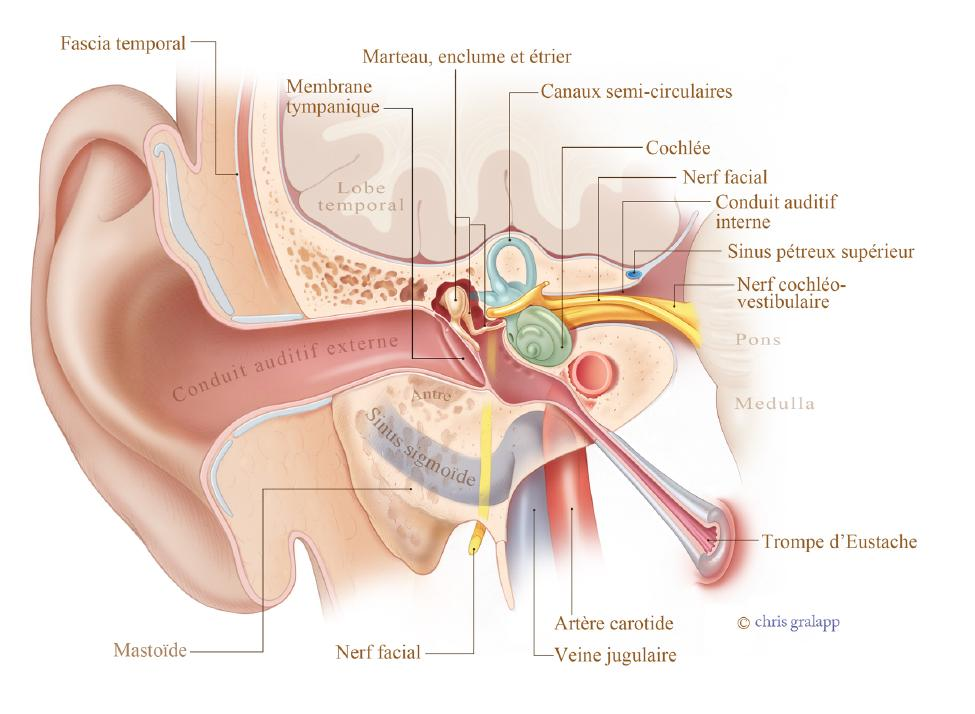
\includegraphics[width=0.7\linewidth]{"images/20160624Berufsfeldgruppen.jpg"}
	\caption[Titre pour toc]{Titre long pour la page}
	\label{fig:-20160624berufsfeldgruppen}
\end{figure}


%\begin{figure}
%
%\caption[Schéma global]
%%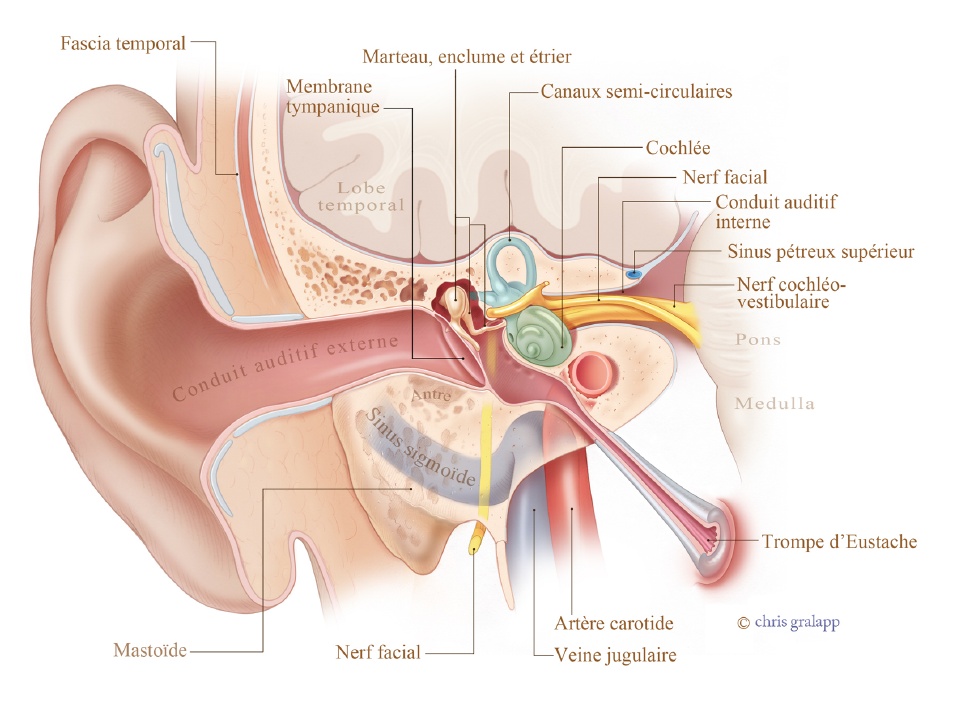
\includegraphics[scale=0.2]{images/20160624Berufsfeldgruppen.png}
%\end{figure}

\paragraph{L'oreille se situe à l'intérieur de l'un des os du crâne, le temporal,
et plus précisément la pyramide pétreuse ou rocher. Elle se compose
de trois parties : externe, moyenne, interne.}
\begin{enumerate}
\item L'oreille externe : formée du pavillon et du méat acoustique externe
(canal auditif). Les ondes sonores entrent dans le méat et percutent
une membrane de 60 mm2, appelée tympan, et la font vibrer. Cette membrane
sépare l'oreille externe de l'oreille moyenne. Selon Tomatis, elle
joue un rôle de filtre des graves et d'amplificateur des aigus.\footnote{Biologie humaine, principes d'anatomie et de physiologie, Elaine N.Marieb,
éd.Pearson Education, 8ème édition, chap. 8, pp.319-321}
\item L'oreille moyenne : se trouve dans l'os temporal constituée de petites
cavités dont une, centrale, qui est la caisse du tympan. Sa limite
médiale est une paroi osseuse percée de deux orifices , la fenêtre
du vestibule et la fenêtre de la cochlée. La trompe auditive ou d'Eustache
est un conduit oblique qui relie l'oreille moyenne à la gorge et sert
à équilibrer la pression de l'air entre l'oreille moyenne et l'extérieur.
Les trois osselets de l'ouïe sont : le marteau, l'enclume et l'étrier
( les plus petits os du corps). Ils transmettent les vibrations du
tympan aux liquides de l'oreille interne. Le marteau et l'étrier sontse
trouve dans l'os temporal constituée de petites cavités dont une,
centrale, qui est la caisse du tympan. Les trois osselets de l'ouïe
sont : le marteau, l'enclume et l'étrier ( les plus petits os du corps);
le marteau et l'étrier sont commandés chacun par un muscle. D'après
Tomatis, son rôle est double : protéger l'oreille interne des sons
trop forts et celui de cibler les sons à écouter.
\item L'oreille interne : est l' organe de l\textquoteright audition. Il
est constitué d'une coque osseuse d'une très grande densité( la plus
importante du corps), contenant un corps membraneux qui en épouse
la forme. L'oreille interne est une enfilade de cavités osseuses portant
le nom de labyrinthe osseux. Il comprend trois subdivisions : la cochlée,
le vestibule du labyrinthe et les canaux semi-circulaires. Le labyrinthe
osseux est rempli de périlymphe, un liquide. Et dans ce périlymphe
flotte le le labyrinthe membraneux qui contient lui-même un liquide
plus épais appelé endolymphe. Ils jouent leur rôle dans l'équilibre
statique et dynamique.Le vestibule et les canaux semi-circulaires
sont les organes de l\textquoteright équilibration , la cochlée ou
limaçon est l'organe de l'audition. 
\end{enumerate}
\begin{quotation}
\char`\"{}C'est le son qui a fabriqué l'oreille et si tu veux connaître
le son, apprends d'abord à étudier l\textquoteright oreille\char`\"{}.
Hermès Trimégiste
\end{quotation}

\subsection{La physiologie de l'oreille : }

Le chemin du son dans l'oreille jusqu'au cerveau : 

Chaque son parvenant à l'oreille entre dans le pavillon et se propage
dans le conduit auditif. Les vibrations de l'onde sonore mettent en
mouvement le tympan lié aux trois petits os (marteau, enclume, étrier).
La transformation (et l\textquoteright amplification) des vibrations
aériennes en vibrations solidiennes se fait par l\textquoteright intermédiaire
des osselets : les vibrations du tympan entraînent successivement
celles du bloc marteau-enclume puis celle de l\textquoteright étrier,
qui les transmet à l\textquoteright oreille interne via la fenêtre
ovale.

Le rapport de levier effectif entre le marteau et l\textquoteright enclume
(de l\textquoteright ordre de 20), d\textquoteright une part, et le
rapport de surfaces entre le tympan (60mm2) et la platine de l\textquoteright étrier
(30 mm2) d\textquoteright autre part font du système tympano-ossiculaire
un véritable amplificateur permettant à l\textquoteright énergie sonore
d\textquoteright être transmise presque intégralement à l\textquoteright oreille
interne.

A partir de 80 dB, un réflexe protecteur (stapédien) est mis en place
afin de réduire la transmission des pressions vers l\textquoteright oreille
interne, par l\textquoteright intermédiaire des osselets et des muscles
qui rattachent le marteau et l\textquoteright étrier aux parois de
la caisse du tympan. Il s'agit ainsi d' un procédé mécanique qui amplifient
les vibrations atteignant la cochlée. 
\begin{quotation}
La cochlée à son tour ``va transformer ces vibrations en impulsions
nerveuses véhiculées par le nerf auditif.'' (...)Les cellules ciliées
tapies dans la membrane cochléaire ``transforment ces vibrations
en messages électriques, circulant dans le nerf auditif. (...) Et
ces informations vont ``se diriger vers le cortex cérébral, via plusieurs
relais.(...) ``Comme certaines fibres issues de chaque oreille croisent
la ligne médiane, chaque aire auditive reçoit des signaux des deux
oreilles.'' De plus, ``tout au long du trajet, le message subit
des transformations dues aux caractéristiques de l'activité des neurones.''
Retenons que `` les cellules ciliées proches de l'étrier sont activées
par les sons aigus, et celles situées au sommet de la cochlée le sont
par les sons de basse fréquence''.(...) `` Une scène auditive est
mêlée d'un ensemble d'ondes acoustiques et son analyse se ferait non
seulement tout au long du système auditif avec des indices comme la
fréquence et l'intensité mais aussi au-delà, pour utiliser les informations
liées aux autres sens ou au contexte.'' \footnote{E.Bigand,\emph{ Le cerveau mélomane}. pp.15-16.Ed.Belin, novembre
2013}
\end{quotation}

\section{Critiques et interrogations :}

Tomatis s'oppose sur plusieurs points aux théories classiques de la
physiologie auditive : 
\begin{itemize}
\item l'oreille moyenne et son rôle de transmetteur 
\item l'analyse fréquentielle au niveau de la cochlée
\end{itemize}
Son originalité réside dans sa conception de la transmission du son
au niveau de l'oreille interne. 

Il propose une nouvelle compréhension de l'oreille, celle-ci étant,
à son regard, un organe actif dans le sens suivant :
\begin{itemize}
\item L'oreille moyenne, grâce aux muscles de l'étrier et du marteau, fait
un travail de visée en ciblant les sons à écouter : le tympan se tend
pour se mettre en résonance avec les sons à percevoir.
\item Il fait aussi un autre travail qui est celui de sélectionner des sons
pour se protéger : la tension tympanique se détend pour amortir l'intensité
sonore qui inonde l'oreille interne. 
\end{itemize}
\begin{description}
\item [{Selon}] la théorie de Georg Békésy, qui obtint le prix Nobel de
physiologie en 1961 et qui reste encore la référence classique, l'oreille
ne sert qu'à transmettre les sons de manière passive comme peut le
faire un micro. Le rôle des osselets se limite à la transmission du
son. Comme déjà décrit plus haut, les sons font vibrer le tympan qui,
étant attaché au marteau, répercute ces ondes acoustiques en mouvements
mécaniques via les osselets. L'étrier transmet ensuite ces mouvements
à l'oreille interne en jouant comme un piston au niveau de la fenêtre
ovale. L'information acoustique est alors transmise sous forme d'ondes
liquidiennes ou encore de tourbillons. Les tourbillons sont analysés(
amplitude et vitesse) en termes de fréquences et de volume par les
cellules ciliées qui tapissent l'oreille interne. 
\item [{Selon}] Tomatis, cette théorie a de nombreuses incohérences. L'une
d'entr' elles serait que cette démonstration ne marche qu'avec un
son pur \footnote{un son pur est constitué d'une unique fréquence ou onde}.
Or, les sons purs n'existent pas dans la nature, car ils sont, au
contraire, complexes et formés d'une multitude de fréquences et d'intensités
variées. Et cette complexité ne peut pas être transmise sans perte
et instantanément par des mouvements mécaniques et retransformée en
tourbillons. De plus, il y a un espace entre l'enclume et l'étrier,
microscopique à l'oeil nu mais énorme sur un plan comparatif, c'est
un hiatus considérable à l'échelle atomique puisqu'il est de l'ordre
d'un millimètre. Ce phénomène reste inexpliquable sur le plan de la
physique pure.
\end{description}
\footnote{Conférence au IIème Congrès International d'Audio-Psycho-Phonologie
Paris 1972 \emph{: Nouvelles théories sur la physiologie auditive}} : il est de l'ordre de s'interroger s'il est possible que la transmission
puisse se faire dans ces conditions. On peut imaginer que le son passe
partout, par les ligaments de jonction des osselets ou les espaces
inter-ossiculaires mais

ce n'était pas scientifiquement prouvable lors d'une de ses conférences
en 1972. Peut-être l'est-il à l'heure actuelle, mais nous n'en avons
pas trouvé trace. 

Nous allons aborder la conduction osseuse qui pourrait nous aider
dans cette compréhension.
\begin{description}
\item [{La}] conduction osseuse : lorsque l'on fait l'expérience de se
boucher les oreilles et de parler normalement, on se rend compte que
notre voix se propage principalement par les os de la tête. Comment
expliquer que l'on perçoive parfaitement bien les sons par conduction
osseuse en mettant un vibrateur conducteur de son sur la boîte crânienne
? et ce, même si l'oreille moyenne est abîmée ( tympan percé, osselets
non fonctionnels) . Selon une dernière recherche, effectivement, le
son stimule l'oreille de deux manières : par voie aérienne en transitant
par les trois parties de l'oreille et par voie osseuse en stimulant
directement l'oreille interne par vibrations des structures osseuses
qui l'entourent. Ce site : oreillemudry.ch a été mis à jour le 28.07.2016.
Il relève l'importance de la voie osseuse mais ne signale aucun nouvel
élément dans la transmission fréquentielle que celle dite classique,
évoquée plus haut. 
\item [{Schéma:}] Physiologie de l\textquoteright audition 
\item [{D'après}] Tomatis, les sons arrivent bien par le canal auditif
jusqu'au tympan. L'onde acoustique excite la membrane tympanique et
par voie de conséquence, l'os de la caisse du tympan. A l'instar d'une
peau de tambour qui fait chanter le bois auquel elle est attachée,
c'est toute la boîte crânienne qui inondée de sons et en particulier
l'oreille interne. Celle-ci, de par sa grande densité, capte les sons
et résonne comme du cristal. (\marginpar{ La transmission du son par l'os est de 5000 m/s.}
Les fréquences qui forment les sons vont ainsi exciter les cellules
ciliées qui tapissent la cochlée, tel un piano enroulé. 
\item [{Avec}] sa théorie, l'analyse multifréquentielle ne se pose plus
: chaque fréquence se dirige instantanément et naturellement\emph{
}vers la cellule ciliée qui lui correspond. C'est grâce à la forme
particulière\emph{ }du limaçon qu'il y a un tri fréquentiel instantané.
Le son identique fréquentiellement s'installe toujours au même endroit
, sur une ligne isofréquentielle, qui est une tranche perpendiculaire
à l'axe.
\end{description}
Et le phénomène des tourbillons n'a donc pas pour fonction de transmettre
les sons mais interviennent pour déclencher les mécanismes d'adaptation
aux bruits. 
\begin{description}
\item [{Comment}] cela se passse-t-il ? Lorsque l'intensité des sons augmente,
l'excitation des cellules ciliées provoque des perturbations liquidiennes
dans l'oreille interne, c.à.dire des tourbillons. Ceux-ci se propagent
et sont amortis par l'étrier. Si les sons atteignent une intensité
dangeureuse pour les cellules ciliées, l'étrier réagit fortement et
entraîne une réaction du marteau qui modifie la tension du tympan.
A son tour, le tympan, relâché, amortit le volume sonore transmis
à l'oreille interne, comme la paupière qui se ferme quand la lumière
est trop intense.
\end{description}

\subparagraph*{``Le tympan se met dans un certain état de tension pour jouer le
rôle d\textquoteright un diapason qui fait vibrer toute la boîte cranienne
par l'intermédiaire du sulcus tympani. \emph{C'est toute la boîte
crânienne qui vibre et qui transmet le son à la vésicule labyrinthique
et non à la chaîne ossiculaire que l'on a l'habitude de considérer
comme le véhicule du son. }La chaîne ossiculaire est un ensemble qui
joue le rôle d'adapteur, de régulateur et non de transmetteur. La
conduction du son par l\textquoteright air puis par l'os doit donc
être étudiée d\textquoteright une façon complémentaire afin que l'on
puisse déterminer par la suite la posture d'écoute du sujet.''\protect\footnote{key 14, Entretien réalisé par B.Auriol avec Tomatis, Anvers 1973}}

Il serait passionnant de faire une étude comparative approfondie des
recherches actuelles au sujet de la physiologie auditive. Génère-t-elle
toujours autant d' interrogations et de débats ?

Christine Petit note et relève par ces recherches le rôle important
et indéniable de la cochlée sur notre audition et spécifie qu'encore
à l'heure actuelle, il reste très mystérieux. \nomenclature{cochlée}{Anatomie : organe de l'audition,appareil sensoriel, en forme de spirale, la cochlée, incluse dans l'os du rocher, forme le limaçon membraneux ,se situe dans l'oreille interne et permet de déceler des sons extrêmement faibles, de discréminer des fréquences et de masquer des sons faibles par des sons forts. }
''C'est une sorte de minuscule appareil électroacoustique capable
de discréminer des sons extrêmement faibles, capable de \emph{masquer
les sons faibles par des sons forts}, pouvant \emph{distordre les
sons,} et en conséquent, \emph{capable d'élaborer un traitement extrêmement
sophistiqué des sons}.''

\footnote{ Christine Petit, titulaire de la chaire Génétique et physiologie
cellulaire au Collège de France, entretien en novembre 2012, réalisé
par Laurent Salters et Vincent Gaullier, Look at science : le système
sensoriel auditif confirme lors d'un entretien réalisé en 2012 le
rôle indéniable de la cochlée. key-13}
\begin{description}
\item [{Observation}] et critiques sur l'application et l'utilisation de
la méthode Tomatis : 
\item [{C'est}] une méthode controversée car il manque des études médicales
de grande envergure sur le sujet, susceptibles d'une évaluation statistique
sûre. Selon Pierre Lane, journaliste de l'émission Envoyé spécial
\footnote{Emission télévisée ``Envoyé spécial''16.5.1991}, Tomatis
a inventé une méthode qui est très critiquée mais qui a donné des
résultats. Elle ouvre l'oreille par des procédés mécaniques pour atteindre
des domaines spécialisés , que ce soit en médecine, en psychologie,
en ostéopathie, etc. Pierre Lane précise qu'il s'agit d'un outil proposé
en complément de leur pratique à de nombreux spécialistes. 
\item [{Au}] fil des années, de nombreuses études scientifques et cliniques
ont été faites. Il est possible d'en trouver le contenu sur le site
internet officiel Tomatis : Tomatis Research and Publication des plus
anciens aux plus récents en 2016.\footnote{www.tomatisassociation.org}
Nous pouvons citer les travaux des Docteur Du Plessis sur l'effet
Tomatis sur l'anxiété en milieu scolaire et universitaire,\footnote{Troubles psychologiques : Etude du Plessis (Université de Potchefstroon
- Afrique du Sud)avec un comparatif Pre / Post niveau d\textquoteright anxiété.
Du Plessis a étudié le cas de 29 étudiants sujets à l\textquoteright anxiété.
10 étudiants ont suivi des séances d\textquoteright écoute Tomatis\textregistered ,
9 ont suivi une psychothérapie classique et 10 ont été choisis pour
former le groupe contrôle. Le groupe Tomatis\textregistered{} a montré
une réduction significative de l\textquoteright anxiété, tandis que
les resultats sont mitigés pour ceux qui ont suivi une psychothérapie
et inexistants pour le groupe contrôle.

Une seconde étude De Plessis a démontré qu\textquoteright après 14,3
mois le niveau d\textquoteright anxiété avait continué à baisser fortement
pour le groupe Tomatis\textregistered{} alors qu\textquoteright aucun
changement n\textquoteright apparaissait pour le groupe contrôle.} \footnote{Du Plessis W.F. and Van Jaarsveld, P.E.(1988), \emph{Audio-psycho-phonology
: A comparative outcome study on anxious primary school pupils, }S\emph{.}Afr.
Tydskr.Sielk.1988,18(4)144-151;

Du Plessis,W.F., Burger,S.(2001)(..) \emph{A pilot study involving
the Tomatis method.}Sud Africa J.Psychol. et plus récemment encore
(2004) \emph{The Impact of a Combined Tomatis and Psycho-Educational
Program on Weight Preoccupied, Female south African Students, }International
Journal of Tomatis Method Research,1(1)54-65} les travaux de Jan Gerritsen, PhD (2009) \footnote{\emph{A Review of Research done on Tomatis Auditory Stimulation}},
les études du dr.P.E.Van Jaarsveld, psychologue à l'Université de
Potchefstroom en Afrique du Sud sur l'action de l'audio-psycho-phonologie
sur le bégaiement \footnote{\emph{The Effect of Audio-Psycho-Phonology on Stuttering}}.
\item [{Plus}] récemment nous citerons encore en dernier lieu la parution
de la dernière recherche menée en collaboration avec le CNRS. Cette
recherche a été publiée dans la revue scientifique \char`\"{}Journal
of Affective Disorders\char`\"{}. Elle a donc fait l'objet d'une validation
par un comité de lecture scientifique. Elle démontre qu'il existe
un lien important et certain entre la difficulté à percevoir certains
sons et l'existence de troubles émotionnels. L'intérêt de stimuler
le cerveau en lui permettant de capter plus facilement ces sons est
donc dès lors évident. Il s'agit d'une étude pilote du Dr.Carlos Escera
de l'Université de Barcelone en 2014 \footnote{\begin{description}
\item [{\emph{http://tomatisassociation.org/scientific-validation-of-the-tomatis-effect-eeg-recordings-of-sound-from-brainstem-to-cerebral-cortex-encoding-university-of-barcelona-2014/}}]~
\end{description}
}sur l'effet d'une technique particulière employée avec l'Oreille Electronique
-la bascule électronique \footnote{( qui permet de créer une alternance entre deux conditions perceptives
du même message sonore -passage soudain et imprévu de fréquences graves
à des fréquences aigues) . }
\item [{Nous}]~
\end{description}
\emph{}\footnote{\emph{``Les seuils auditifis des sons purs sont diminués chez les
personnes déprimées avec des troubles de stress post-traumatique.''}
\begin{description}
\item [{\emph{\char`\"{}Pure-tone}}] \emph{auditory thresholds are decreased
in depressed people with post-traumatic stress disorder\char`\"{}
Journal of Affective disorders.} Recherche du CNRS en collaboration
avec Tomatis Developpement S.A.
\end{description}
Auteurs : Stéphanie Aubert-Khalfa; Emmanuelle Reynaud; Myriam El Khoury;
Olivier Blin - INCM, UMR CNRS 6193, Jean-Pierre Granier - TOMATIS
DEVELOPPEMENT S.A. Eva-Maria Grosse; Jean-Claude Samuelian - Pôle
Psychiatrie Centre, La Conception Hospital }

Il y a lieu d'observer et de remarquer que certaines de ces études
ont été menées en collaboration avec la société Tomatis actuelle,
ce qui enlève quelque peu l'intégrité de la recherche.
\begin{quotation}
Selon le Dr.med.Inge Flehming\footnote{Dr.med.Inge Flehming, neurologue, neuropédiatre, texte publié en allemand
en 1996,\emph{``Grundsatz-Gutachten zur Behandlungsmethode nach Prof.Tomatis''http://www.analytische-hoertherapie.de/uploads/tx\_templavoila/Grundsatzgutachten\_zur\_Behandlungsmethode\_nach\_Prof.\_Tomatis.pdf}}''il est compréhensible que les médecins ORL n'en soient pas convaincus
par le fait que les objectifs thérapeutiques sont différents. L'ORL
cherche à améliorer l'audition tandis que le neurologue ou le neuropédiatre
ne s'en préoccupe pas, mais cherche à comprendre les raisons pour
lesquelles certains sujets ont des difficultés à appréhender ce qu'ils
entendent, c'est-à-dire à traiter correctement l'information au niveau
du cerveau.''
\end{quotation}
\begin{quote}
\footnote{``Or le traitement central correct d'un stimulus relayé au cerveau
par les voies sensorielles présuppose l'acquisition d'une synergie
parfaite entre les systèmes sensoriels au niveau de l'organe central
(le cerveau), un processus nommé \char`\"{}intégration sensorielle\char`\"{}.
Dans ce contexte, Tomatis distingue entre \char`\"{}l'audition\char`\"{},
prise comme l'expression de la réalisation acoustique de l'impulsion
auditive dans le cerveau, et \char`\"{}l'écoute\char`\"{}, prise comme
un processus \char`\"{}d'écoute consciente\char`\"{}, impliquant l'attention
immédiate et la conscience subjective de l'individu. En présence d'une
stimulation adéquate, toutes les voies sensorielles du corps sont
en mesure de réaliser l'intégration sensorielle, prise comme synergie
des systèmes sensoriels, et leur interconnexion au niveau du cerveau.
L'oreille joue néanmoins un rôle tout à fait particulier dans ce processus.
En effet, le labyrinthe osseux de l'oreille interne réunit deux systèmes
sensoriels diamétralement opposés, mais néanmoins fondamentaux, l'un
et l'autre, dans un espace très réduit. Le système auditif est le
premier système sensoriel achevé sur le plan anatomique dans l'évolution
prénatale de l'enfant. Cela veut dire que dès une phase précoce de
la grossesse, l'audition est entièrement opérationnelle, et mise à
contribution. De nos jours, nous savons que la formation de synapses
entre les neurones du cerveau, c'est-à-dire le câblage et l'interconnexion
des milliards de neurones présents dans le cerveau, obéit à un processus
activement contrôlé, où des dendrites \char`\"{}chercheurs\char`\"{}
et des dendrites \char`\"{}récepteurs\char`\"{}, guidés en-cela par
des molécules dits \char`\"{}neuro-tactiques\char`\"{}, établissent
des liens persistants avec une précision tout à fait remarquable.
Ces liens, qui sont d'une importance vitale pour l'individu, resteront
pour la plupart en place pendant toute sa vie. Ce processus de formation
de synapses ou d'interconnexion des neurones débute chez l'enfant
dès les premières semaines de la grossesse. Il est d'ailleurs stimulé
par la sollicitation active des organes sensoriels. Dans ce contexte,
et à juste titre, Tomatis souligne l'importance du développement sensoriel
prénatal de l'enfant. Il affirme que l'audition précoce, intra-utérine
de l'enfant, joue un rôle moteur pour le développement de tous les
systèmes sensoriels de ce dernier, leur permettant de fonctionner
en synergie, de former un réseau de connexions cérébrales dès un âge
précoce, à savoir longtemps avant la naissance, favorisant ainsi la
maturation du cerveau dans son ensemble.''(...)L'influence réciproque
entre les systèmes auditif et vestibulaire ne se limite pas à la proximité
spatiale des deux organes dans l'oreille interne. En effet, il y a
des connexions centralisées au niveau du cerveau entre le nerf acoustique
et d'autres facultés sensorielles, qui touchent bien évidemment aussi
l'organe de l'équilibre. (résultat de frayeur et réaction de fuite
dûe à un bruit : un enchaînement de réflexes liés à la fois à la proprioception
et au système vestibulaire. C'est tout le corps qui réagit en esquissant
une réaction de fuite.'' (...)}
\end{quote}
\begin{quotation}
(...)``La thérapie selon Tomatis, en ce qu'elle influence les mécanismes
de la perception auditive, a un effet bénéfique global, holistique,
qui n'opère pas tant sur l'audition que sur l'écoute attentive, la
régulation de la tonicité musculaire, la coordination entre la motricité
globale et la motricité fine, et l'érection de l'individu dans l'espace.
Bien évidemment, ce sont des aspects auxquels les neurologues du développement
ou neuropédiatres sont plus sensibles que les ORL, dont les objectifs
s'inscrivent dans un tout autre domaine. La thérapie selon Tomatis
ne relève pas de la médecine alternative, ni de l'ésotérisme, mais
d'une neurophysiologie appliquée et holistique ; à ce titre, elle
joue un rôle tout à fait marquant.''\footnote{Dr.med. Inge Flemming}
\end{quotation}
Force nous est de constater que cette même forme de controverse existe
aussi avec d'autres types de thérapies telle l'acupuncture, bien qu'ancestrale
et riche de résultats : les mécanismes en jeu étant non élucidés et
les études d'évaluation encore insuffisantes. 

La neuroscience nous apporte beaucoup dans le domaine du cerveau et
de la musique. Rien n'est encore élucidé. Peut-être ces recherches
aboutiront-elles avec des résultats qui prouveront cette méthode ou
la démonteront ? Pour l'instant, sans preuve scientifique à l'appui,
nous continuons à investiguer dans les critiques.

D'autre part, comme pour tous types de thérapies, la qualité de prise
en charge varie également avec la qualité du médecin ou du thérapeute.
Ceux-ci ne sont pas forcément à la hauteur des attentes du patient
qui doit toujours garder un esprit critique.

Un des reproches tout à fait justifié de la méthode Tomatis est parfois
le manque de suivi. Le patient se trouve un peu ``largué'', avec
une oreille remise au point mais avec laquelle il se sent perdu. Il
faut du temps pour qu'il puisse s'y habituer et que les nouvelles
façons de fonctionner s'intègrent. L'accompagnement du patient dans
la phase active nécessite du temps. L' investissement est différent.
Nous rentrons de plein fouet dans le domaine de compétences des champs
d'application des thérapeutes.Ce peut être celui des logopédistes
par exemple, ou des musicothérapeutes.

\section{Technique de travail sous ``Oreille électronique'' :}

Dès 1952, comme preuve et application des trois lois qu'il avait énoncées,
Tomatis a concentré ses efforts de recherche sur la mise au point
d'un appareil susceptible de mondifier la manière d'entendre et, par
voie de conséquence, la façon de parler d'un sujet. Par cet appareil,
le but était d'obliger l'oreille à utiliser un mode d'accomodation
déterminant une manière d'entendre typique et entraînant le geste
vocal correspondant.

Conçue déjà en 1947, L'Oreille Electronique est ``la réplique parfaite
d'une oreille humaine'' nous dit son inventeur. L'oreille parfaite
saurait écouter ; elle passe de l'entendre à écouter, elle se tend
vers l'information qui lui arrive. Ce n'est pas si facile, ce n'est
pas inné. Et si on met l'Oreille électronique en parallèle avec une
oreille qui ne rentre pas dans cette dynamique, elle va l'entraîner.
Elle sert à faire faire une gymnastique bien précise ou un jeu de
contractions.

L'adaptation de l'oreille moyenne se fait par le jeu des contractions
du muscle du marteau et du muscle de l'étrier.
\begin{itemize}
\item Le muscle du marteau agit sur la convexité imposée au tympan, qui
se comporte alors comme une lentille acoustique, sorte de cristallin
auditif.
\item Le muscle de l'étrier régule le jeu de l'oreille interne, qui sait,
à la manière d'un prisme, étaler la gamme des sons en spectre acoustique.
\end{itemize}
Cette accomodation plus ou moins rapide, plus ou moins complexe, permet
d'ouvrir telle ou telle bande passante auditive, d'agrandir selon
les besoins, le diaphragme d'ouverture.

L'Oreille Electronique impose ce jeu à l'oreille.

ll y aura un travail dit ``passif'' dans le sens que ce sera d'abord
un travail d' écoute de musiques et un travail dit ``actif'' où
la personne s'implique directement en émettant des sons avec la possibité
de travailler et d'être corrigé immédiatement sous Oreille Electronique.

Dans le but de faire faire cette gymnastique microscopique aux muscles
de l'oreille, ces musiques peuvent être préparées avec un jeu de bascule{*}(
cf explication 3.3.3.) qui alterne le passage des basses aux hautes
fréquences; elles peuvent aussi l'être avec un certain pourcentage
de filtrages \footnote{}qui va varier et s'ajuster selon la personne
et le résultat des tests d'écoute. Pour stimuler le désir d'écoute
du patient, il est aussi possible de préparer des musiques avec une
technique particulière, dénommée retard, agissant sur le muscle de
l'étrier, c'est-à-dire sur la conduction osseuse. Une autre technique
est celle de la précession, qui aidera à viser et décoder les messages,
en agissant sur le tympan, c'est-à-dire sur la conduction aérienne. 

Ce type de traitement n'est donc pas le fruit du hasard mais d'une
longue recherche pour la mise au point de ces différentes techniques
sous Oreille Electronique.

\section{Travail ``passif'' et ``actif''sous Oreille Electronique}

\subsection{Technique dans le travail passif et actif : }
\begin{itemize}
\item La façon générale de procéder est l'alternance d'écoute de musiques,
de travail actif avec la voix, de tests d'écoute, de pauses.
\end{itemize}
Avant les séances : un test d'écoute, focus sur l'audition avec un
graphique.

Après les séances : le même test, avec visualisation d' une évolution
ou d'une transformation de l'écoute du patient : un changement sera
visible ou ne le sera pas.

\subparagraph{Dans le travail passif : }
\begin{description}
\item [{1\textdegree Session}] de 25 à 30h d'écoute : le patient écoute
deux heures de musique par jour pendant 13 à 15 jours consécutifs;
un deuxième test à la fin de ce travail; ensuite, une pause pendant
4 à 6 semaines.
\item [{2\textdegree Session}] de 25 à 30h d'écoute : 3ème Test, à nouveau
deux heures d'écoute pendant 13 jours à 15 jours; puis 4ème test,
suivi d'une pause d'une durée de 4 à 8 semaines.
\item [{3\textdegree Session}] : la même façon de procéder que les deux
autres. 
\end{description}
Le choix et le traitement des musiques peuvent être très différents
selon le patient et sa pathologie.

But du travail passif : \emph{``}Ouverture\emph{'' }de l'oreille
aux sons : sensibiliser à certains sons avec l'objectif de réintégrer
des fréquences perdues ou annihilées inconsciemment ou volontairement. 

Cette technique de travail se sert du son pour provoquer un résultat
physiologique. Elle dérange les habitudes d'écoute pour faire agir
et ré-agir le patient. Cette phase est parfois totalement rejetée
par le patient.

\subparagraph{Dans le travail actif :}

Après avoir été stimulé et ouvert aux sons environnants, le patient
est amené par le thérapeute à travailler sa voix. On cible un travail
actif de la voix à l'aide des écouteurs spécifiques de la méthode
car la correction de la voix y est instantanée et instaure les bons
réflexes de la boucle audio-vocale. C'est un processus naturel par
lequel l'individu assimile et analyse l'information sonore qu'il reçoit
et ajuste en retour l'information sonore qu'il émet. Le patient va
commencer à s'en servir ``à volonté'', c'est-à-dire d'ajuster et
d'analyser ce va-et-vient permanent entre l'écoute et l'émission vocale
afin de créer une forme de réflexes sur lesquels il peut ``s'asseoir''. 

Cette phase de la thérapie est importante et parfois très délicate
pour le patient. Accepter d'entendre sa propre voix n'est pas toujours
simple et l'encadrement et le soutien sont nécessaires pour permettre
au patient de franchir cette étape. Lorsqu'elle se passe bien , il
y a en quelque sorte réintégration de la voix dans le corps. Le patient
apprend à créer lui-même cette boucle phonatoire sur laquelle il va
pouvoir se reposer, se ressourcer, se régénérer pour être totalement
autonome au bout de sa restructuration : une reprise en main qui va
lui permettre d'``être et de se sentir auteur de sa propre vie''. 

\subparagraph{\textmd{\emph{``L'émission vocale confirme et reconfirme à chaque
fois le sujet dans son intégrité et son identité.''A.Tomatis}}}

\footnote{Tomatis en fait une description précise dans la troisième partie de
son livre\emph{ L'oreille et la voix, pp.185-301}}

Vu et décrit sous un oeil scientifique, ``il existe une interaction
constante entre le traitement auditif et le traitement moteur de la
voix, entre l'information sensorielle et les programmes moteurs impliqués
dans la parole ou le chant. Le programme moteur qui a été déclenché
pour la parole permet au cerveau de faire des hypothèses constantes
sur les conséquences acoustiques du geste vocal qui est sur le point
d'être réalisé. Ensuite, l'hypothèse est comparée à l'information
auditive reçue. C'est principalement à travers l'activation de la
boucle audio-vocale que peu à peu, le cerveau va modifier l'hypothèse
qu'il a construite à propos des conséquences acoustiques du geste
vocal sur le point d'être réalisé.'' \footnote{J.P.Granier, Tomatis Développement,\emph{ Conférence Paris}, 13.5.2012}

\chapter{La musicothérapie et la psychothérapie}
Nous savons que la musicothérqpie est de plus en plus intégrée dans les milieux psychiatriques.
Comme il s'agit du domaine dans lequel je travaille et que j'ai choisi d'analyser pour ce travail, nous aimerions traiter plus précisément des sujets de la dépression et du burn-out, très  souvent associés.


\chapter{La dépression}

\chapter{Le test Tomatis : }

\section{Explication :}

Tomatis a mis au point un test spécifique destiné à fournir une traduction
graphique de l'écoute.

Ce test est fait pour :
\begin{itemize}
\item constater la posture d'écoute de la personne ainsi que l'articulation
des trois systèmes : la fonction de dynamisation, la fonction vestibulaire,
et la fonction d'écoute.
\item observer les modifications et les évolutions des courbes au cours
de la thérapie.
\end{itemize}
Tomatis était un médecin O.R.L, un clinicien car ses constatations
sont issues d'observations et de résultats ; il a commencé en faisant
des tests d'écoute traditionnels, dits objectifs\footnote{Déjà ici, selon les attentes des personnes testées, les résultats
variaient, liés à la peur de perdre un emploi ou à l'obtention d'un
congé maladie.}, avec des observations particulières à des troubles de l'oreille,
comme le scotome, lésion pathognomonique (qui est le terme spécifique
d'une maladie en médecine). 

Un bref retour en arrière : en 1947, il dirigeait le Laboratoire d'acoustique
des arsenaux de l'aéronotique et devait examiner l'audition détériorée
des personnes travaillant sur les bancs d'essais des réacteurs supersoniques.
Tomatis constata que les pertes auditives étaient accompagnées d'une
déformation assez nette de la voix. En travaillant par la suite avec
un patient chanteur, il observa une lésion de l'oreille similaire
à celles observées chez les ouvriers des arsenaux. Il était totalement
vain d'essayer de soigner ce chanteur avec des doses de sulfate de
strychnine, selon les prescriptions habituelles des phoniatres de
l'époque. Aucun résultat n'était obtenu en tendant les cordes vocales
comme un violon qu'on accorde. Il émit alors l'hypothèse fondatrice
que la perturbation de la voix n'était pas due à un défaut des cordes
vocales mais à une détérioration de l'oreille. En fait, ce chanteur
souffrait de surdité professionnelle. Il commença alors à approfondir
ce parallélisme constant entre l'examen audiométrique et la courbe
d'enveloppe de l'analyse des fréquences de la voix. Puis il eut l'idée
d'essayer de corriger la voix défectueuse en imposant à l'oreille
une courbe de réponse auditive idéale. Pour réaliser cette stimulation
de l'oreille, il mit au point un appareil électronique appelé Oreille
Electronique ou appareil à ``effet Tomatis''. Et, dès les premières
séances, il constata une amélioration temporaire de la voix qui devint
peu à peu permanante avec de l'entraînement. 

Tomatis a défini la «courbe d\textquoteright écoute idéale» après
bien de nombreuses expériences sur des personnes qui souffraient de
problèmes de perception auditive. Elle correspond à l'oreille absolue
des chanteurs et des musiciens. Tomatis étudia le ténor italien Enrico
Caruso (1873-1921) dont il analysa la voix à partir des enregistrements
de ses vocalises sur vinyles. Caruso représentait la courbe auditive
optimale. Il utilisa donc sa voix pour élaborer la courbe idéale ainsi
surnommée «courbe de Caruso».

Sur le plan de la physique pure, elle indique les réponses de l'oreille
lorsque celle-ci fonctionne bien. Elle répond en fait à la courbe
de Wegel dite \char`\"{}courbe en citron\char`\"{}, inversée.\footnote{Effectivement la courbe de Wegel est la courbe de réponse obtenue
lorsque sont posées en abscisses les fréquences, et en ordonnées ascendantes
les intensités. Un premier seuil s'obtient, en partie basse, suivant
un minimum qui commence dans les fréquences graves à environ 40-50
dB, avoisine ensuite la courbe des abscisses entre 2000 et 3000 Hz
et redevient ascendante à 40 / 50 dBs dans les aigus entre 8 000 et
10 000 Hz. Cette courbe se complète et prend l'allure de citron selon
l'expression qu'on lui confére lorsqu\textquoteright on envoie des
sons d'intensité croissante et qu'on obtient alors une courbe des
seuils maxima qui se déterminent là où l'oreille commence à souffrir,
d'où le nom de \char`\"{}seuil de la douleur\char`\"{}.Ces seuils
commencent dans les graves, également à 50-60 dB rejoignant la première
courbe, puis ils atteignent 120 à 130 dB entre 2000 et 3000 Hz pour
chuter ensuite dans les aigus en rejoignant également la première
courbe. La ligne médiane qui se situe aux environs de 50-60 dBs, qui
est linéaire représente une zone dite \char`\"{}Zone de Munsen''.
Elle répond à la dynamique de l\textquoteright oreille, c\textquoteright est
à dire à sa zone \char`\"{}optimale\char`\"{} de fonctionnement sans
distortion. Dans toutes les autres zones, l\textquoteright oreille
agit comme un filtre dont les pentes sont variables en fonction de
l\textquoteright intensité, avec un lieu de rotation situé entre 1000
et 2000 Hz. Pour pallier ces distorsions toujours difficiles à intégrer
dans la lecture des schémas, les Américains ont standardisé les audiogrammes
du type de ceux que nous utilisons tous en inversant l\textquoteright image
de Wegel et en redressant les minima pour obtenir une ligne droite.
Ces normes gardent néanmoins une zone préférentielle entre 1000 et
2000 Hz malgré les compensations de 30 à 40 dB accordées sur la courbe,
dans les graves et les aigus.}

L'acquisition de cette courbe idéale correspond à l\textquoteright harmonisation
du jeu de deux muscles de l\textquoteright oreille moyenne. Ce jeu
permet de régler en permanence la pression interne de la vésicule
labyrinthique en faisant intervenir les phénomènes de moindre impédance.
\footnote{Définition de l\textquoteright impédance : L'impédance acoustique
caractérise la résistance qu'un milieu oppose à sa mise en mouvement
lorsqu'il est traversé par une onde acoustique. Elle est définie comme
le rapport de la pression acoustique sur la vitesse de déplacement
locale dans un milieu, et est généralement notée Z. Elle dépend de
la température. L'impédance caractéristique d'un milieu (solide, liquide
ou gazeux) est définie comme le rapport de la pression acoustique
sur la vitesse de déplacement en milieu ouvert (c\textquoteright est-à-dire
en l'absence d'ondes réfléchies). L'impédance caractéristique est
une propriété du matériau considéré égale, dans le cas d'un espace
illimité, au produit de la masse volumique du matériau \textgreek{r}
par la vitesse du son c dans ce même matériau : Z = \textgreek{r}
. c

{[}Unités : \textgreek{r} étant exprimé en kg/m3, c en m/s, Z est
exprimé en Pa.s/m.{]} Lorsqu'une onde acoustique rencontre l'interface
séparant deux milieux d'impédances acoustiques différents, une partie
de l'onde est transmise dans l'autre milieu tandis qu'une autre partie
se réfléchit sur l'interface. On cherchera à estimer les quantités
d'énergie acoustique transmises et réfléchies.

Les ondes incidentes ( f1 ) sont transmises pour une part au second
milieu ( f2 ) et pour une autre part, elles sont réfléchies à l\textquoteright interface
entre le premier et le deuxième milieu jaune ( g1 ) (modifié d\textquoteright après
Wikipedia, 9 février 2009) }

L\textquoteright audiogramme classique donne une courbe déterminée
mais n\textquoteright indique pas pour autant si l'individu examiné
sait vraiment se servir de cette courbe pour communiquer avec les
autres au travers de son autocontrôle.

Son test permet justement de connaître l'utilisation que sait faire
un sujet de son audition.Un oeil anatomiquement parfait ne permettra
pas de déceler si le sujet sait s'en servir en visant au fusil ou
en faisant de la peinture. Toutes les nuances de couleurs qui permettent
au peintre de s'exprimer ne sont pas celles que tout un chacun voit.\footnote{Conférence, Anvers,1973.}
``L'écoute est à l\textquoteright oreille ce que la vision est à
l'½il.'' Il existe donc ``une dimension de gnosie qui apporte une
donnée complémentaire,(...) une dimension d'attention, d\textquoteright adhésion
qui s'institue dans l'écoute, prise de conscience qui s\textquoteright imbrique
à l'audition elle-même.'' 
\begin{quotation}
``Lorsque l'interprétation mentale des informations sensorielles
transmises par l'oreille est erronée, l'écoute est perturbée.''\footnote{\emph{source site officiel Tomatis.com}}
\end{quotation}
Il s'agit de distorsions d'écoute. Cette distorsion est liée au dysfonctionnement
des deux muscles de l'oreile moyenne. Leur rôle est de permettre l'arrivée
harmonieuse du son dans l'oreille interne, puis au cerveau. Car, lorsque
le message sensoriel est altéré, le cerveau se protège en déclenchant
des mécanismes d'inhibition de l'écoute.'' Tout enfant peut naître
avec ce potentiel mais celui-ci s' altére parfois avec les difficultés
de la vie. Il se ferme au monde de l'écoute et il introduit des distorsions
pour se défendre contre les agressions du monde extérieur. 

Sur le plan du test d\textquoteright écoute,\emph{ }on remarquera
alors des distorsions, des manques\emph{ }par rapport à la courbe
idéale qui se trouve sous-jacente dans tout individu. 
\begin{quotation}
``La présence d'une \emph{pente ascendante} est nécessaire pour que
l'oreille puisse bloquer les fréquences graves, les atténuer, afin
que la partie proximale de la cochlée soit utilisée, plus particulièrement
dans la zone consacrée au langage. Ceci est spécifique de l'oreille
humaine. Les auditions de certains animaux sont quant aux bandes passantes,
beaucoup plus développées que la nôtre : le dauphin, par exemple,
entend jusqu\textquoteright à 200.000 Hz, certaines chauve-souris,
certains vampires jusqu'à 150.000 Hz ; un chien entend jusqu'à 45.000
Hz. Mais ce sont là des performances qui représentent peu de chose
par rapport à la faculté qu'a l'oreille humaine d\textquoteright entendre
le langage. Et cette partie d'analyse fine exige qu'elle ne soit pas
gênée par la perception des fréquences graves. (...)''\footnote{\emph{Entretien de Tomatis par Auriol,} Anvers 1973}
\end{quotation}
\begin{quote}
\emph{``L'oreille a un psychisme.''} 
L'intégration de l'audio-thérapie et/ou de la musicothérapie a tout son sens dans le contexte ou le milieu psychiatrique. Tomatis, à notre sens, ne pouvait faire meilleure boutade
\end{quote}
De cette phrase sous forme de boutade, qui nous semble à priori exagérée,
nous pouvons cependant nous interroger sur la récente parution d'un
article d'une étude franco-américaine scientifique \footnote{\emph{Etude scientifique menée au CNRS par l'acousticienne Claudia
Fritz de l'Institut Pierre et Marie Curie,}https://lejournal.cnrs.fr/diaporamas/stradivarius-la-fin-dun-mythe} au sujet des Stradivarius : elle semble ne pas lui donner totalement
tort et même l'atteste d'une autre manière : nous transformons l'écoute
selon nos attentes. Faite avec un protocole d'écoutes en aveugle avec
des violonistes professionnels et en parallèle avec un public (caché
derrière un rideau), cette étude démontre que le mythe de la suprématie
de ces instruments extrêmement chers est tombé au profit d'instruments
neufs. L'étude prouve que le cerveau transforme les informations reçues
selon les attentes que l'on a. Le rôle du cerveau dans notre perceptions
est extrêmement fort et cette étude le prouve scientifiquement. \footnote{http://www.lemonde.fr/culture/article/2014/04/10/le-stradivarius-detrone-par-les-violons-modernes\_4398681\_3246.html }

\footnote{Patrick Dumas de la Roque \emph{``L'écoute, c'est la vie''}p.43.Ed.
Jouvence, collection Trois Fontaines}

\section{Description de la passation du test d'écoute :}

Pour effectuer ce test, un appareil contenant un générateur de fréquences
appelé \char`\"{}Hearing Test\char`\"{}, émet des sons purs s'étalant
de 125 à 8000 hertz, d'octave en octave, en passant par les valeurs
1500 hertz, 3000 et 6000 hertz, et dont l'intensité, peut varier de
5 en 5 dbs, de 10 à + 100 dbs. 

Ce test a pour but de déterminer les 4 paramètres suivants : 
\begin{itemize}
\item a) Recherche des seuils :
\end{itemize}
Il s'agit de rechercher d'une part les seuils d\textquoteright audibilité
minima : il est demandé au sujet de lever de lever la main du côté
où il entend le son, de lever les deux mains lorsqu'il entend le son
des deux côtés ou lorsqu'il ne peut en déterminer la provenance.

Il existe deux types de conduction sonore, l'une aérienne et l'autre
osseuse.

En conduction aérienne, le son pénètre dans le conduit externe de
l'oreille par l'intermédiaire d'écouteurs. Les vibrations du tympan
parviennent à l'oreille interne qui informe le nerf auditif.

En conduction osseuse, le son pénètre à l\textquoteright aide d'un
vibrateur qui vient exciter la mastoïde. Par l'intermédiaire de la
boîte crânienne, les vibrations informent le nerf auditif.

Les résultats sont consignés sur deux grilles correspondant à la courbe
de l'oreille droite et à celle de I\textquoteright oreille gauche.
\footnote{Suivant le processus d'observation habituellement appliqué en physiologie,
la place de ces deux diagrammes est inversée, la courbe droite étant
à gauche et la courbe gauche étant à droite. }

En abscisses, on porte les fréquences de 125 à 8000 Hertz, et en ordonnées,
les intensités en décibels qui se lisent de haut en bas. 

Les seuils reportés sur les graphiques sont reliés entre eux et vont
dessiner deux courbes distinctes : 

-la courbe aérienne (CA) et - la courbe osseuse (CO) de l'oreille
droite et celles de l'oreille gauche.

\footnote{\begin{itemize}
\item Tomatis a volontairement décalé les étalonnages des deux courbes (aérienne
et osseuse) pour pouvoir distinguer les différentes réponses et interpréter
les distorsions. Lorsque l\textquoteright écoute est parfaite, les
courbes aérienne et osseuse se confondent mais pour l'analyse des
résultats, on a déterminé des courbes parallèles, la courbe aérienne
devant être au dessus de la courbe osseuse.
\end{itemize}
}
\begin{itemize}
\item b) Etude de la spatialisation :
\end{itemize}
Lors de la recherche des seuils, on note en même temps le pouvoir
de l'oreille de localiser les sons dans l'espace. On recueille les
confusions ou inversions latérales de sons. Les inversions ou les
confusions de sons sont notées au niveau de chaque fréquence par un
petit trait placé au bas de chacune des grilles. La spatialisation
est un indicateur du degré d'élaboration de la latéralité auditive,
elle donne des repères sur la façon dont le patient intègre les informations
au niveau du cortex, les faisceaux homo et hétéro-latéraux devant
être fonctionnellement différenciés. Les erreurs reflètent la confusion
de cette intégration et donnent une indication sur la latence et l'incertitude
dans le traitement de l'information. ( la manière d'appréhender le
son dans l'espace). Ce peut être la difficulté du sujet à fixer son
écoute, une mauvaise coordination, un manque de confiance en soi ou
une mauvaise organisation des idées.
\begin{itemize}
\item c) Etude de la sélectivité : 
\end{itemize}
La sélectivité est la « faculté que possède une oreille de percevoir
une variation de fréquences à l'intérieur d'un spectre sonore, et
de situer le sens de cette variation »\footnote{\emph{L'oreille et la voix,}A.Tomatis, Ed.Laffont}.
Le but est de déceler l'ouverture ou la fermeture de cette sélectivité
auditive. Pour le faire, on effectue pour chaque oreille, en conduction
aérienne, et à un niveau d'environ 40, 60 décibels, un balayage des
fréquences en partant généralement des aigus. On demande au sujet
d'indiquer si le son perçu est plus aigu, plus grave ou de même hauteur
que le précédent. Les erreurs sont indiquées au niveau des fréquences
mal analysées et le blocage de la sélectivité est indiqué en traits
hâchurés à partir de la fréquence la plus grave qui a été marquée
d'un trait. La sélectivité permet de donner des informations sur la
qualité d'écoute avec trois aspects : au niveau linguistique ( conscience
phonémique), cognitif ( fonctions exécutives) et émotionnel ( action
efférente, présence d'anxiété).
\begin{itemize}
\item d) L'audiolatérométrie : 
\end{itemize}
On recherche la latéralité du patient : droite ou gauche. La dominance
de l'oreille droite comme oreille directrice doit être manifeste.

Ainsi, après la passation du test d\textquoteright écoute, nous nous
trouvons en présence de deux grilles contenant chacune deux courbes,
en général, de deux couleurs différentes complétées par l'indication
des inversions ou confusions de sons, par des données sur la sélectivité
et en même temps par des chiffres qui correspondent à l'épreuve d'audiolatéromètrie.

Les résultats du test permettront de faire une comparaison avec la
courbe dite idéale : c'est une courbe ascendante entre 500 et 2000
hz qui correspond à une pente d\textquoteright environ 6 à 18 db/octave,
puis un dôme entre 2000 et 4000 Hz et ensuite une légère descente. 

\paragraph{Les trois zones du test d'écoute : }

Mise en évidence de différentes zones à l\textquoteright intérieur
de chaque diagramme. 

Ces bandes sonores se répartissent en trois zones, des fréquences
graves aux aigues, de la façon suivante :
\begin{itemize}
\item Zone 1 : de 125 à 1000 Hz : les graves, la zone vestibulaire
\item Zone 2 : de 1000 à 3000 Hz : les mediums, la zone du langage
\item Zone 3 : de 3000 à 8000 Hz : les aigus, zone cochléaire
\end{itemize}

\subparagraph*{Pour notre étude, nous allons nous en tenir à celui de la recherche
des seuils : seuil de la courbe aérienne et seuil de l'osseux des
deux oreilles, gauche et droite.}

\section{Interprétation du test : }

\subsection{Signification et interprétation psychologique du test : }

\paragraph{La première étape : une approche globale : }

Ce sont des comparaisons graphiques des courbes. 

On considère l'allure générale des courbes, on compare leur dessin
: la forme des courbes, l' équilibre, la symétrie ; et on étudie leurs
rapports entre eux : 

courbe aérienne (CA) - courbe osseuse (CO) - rapport entre CA et CO
pour chaque oreille - rapport entre CA et CO d\textquoteright une
oreille à l'autre. si ce rapport est correct, CA est placée au-dessus
de CO sur la grille.

\subparagraph{Les deux types de courbes véhiculent chacune des informations spécifiques
sur la posture d'écoute du sujet : }
\begin{itemize}
\item La conduction aérienne : traduit la vie sociale, la manière de communiquer
et de s'extérioriser, permet de préciser la façon dont le sujet\emph{
écoute le monde extérieur} et en particulier l\textquoteright autre,
son interlocuteur, celui qui lui parle. 
\item La conduction osseuse : traduit la vie intérieure, mode de fonctionnement
organique, d'une façon générale : liée aux tensions.C'est la courbe
de l\textquoteright auto-écoute, de l\textquoteright auto-contrôle,
de l'écoute intérieure.
\end{itemize}

\subparagraph{Les courbes donnent des informations selon leur ascendance, leur
continuité et leur similarité oreille droite/ oreille gauche.}
\begin{itemize}
\item Continuité de la courbe : Si une courbe est continue, elle définie
comme harmonieuse et ne comporte pas de pics ou de scotomes qui laisseraient
supposer l'existence de nombreuse tensions.
\end{itemize}
Situées en CO, ce sont des tensions internes non exprimées : attitude
calme mais très tendue intérieurement.

Situées en CA, ce sont des tensions réelles et exprimées au quotidien
: soit somatisées, soit verbalisées ou soit manifestées sur le plan
affectif (pleurs).

\subparagraph{Les trois zones du test d'écoute : }
\begin{itemize}
\item Zone 1 : de 125 à 1000 Hz : les graves, la zone vestibulaire, élaboration
du schéma corporel, des repères temporo-spatiaux, adresse motrice,
esprit pratique.
\item Zone 2 : de 1000 à 3000 Hz : les mediums, la zone du langage, de la
verbalisation, compréhension, mémorisation, de l'intégration des lois/
des règles, esprit analytique.
\item Zone 3 : de 3000 à 8000 Hz : les aigus, zone cochléaire, de l'énergie,
de l'imagination, de l'expression, motivation, esprit synthétique.
\end{itemize}

\subparagraph{Les trois zones de fréquences du test d'écoute correspondent à des
caractéristiques précises ; et, avec l'allure des courbes, on doit
tenir compte de leurs particularités.}

Lorsqu'une zone du test d'écoute est nettement dominante et semble
traduire une caractéristique de la personnalité, on peut situer un
sujet dans un registre particulier correspondant à son tempérament.

- courbe accentuée dans la zone fréquentielle des graves : tempérament
somatoïde, orienté vers le corps

-courbe accentuée dans la zone fréquentielle des médiums : tempérament
paranoïde, attaché à la logique, la règle, le raisonnement 

-courbe accentuée dans la zone fréquentielle des aigus : tempérament
schizoïde, reflétant une recherche de créativité.

\subparagraph{Signification des diagrammes droite et gauche : }

Tout ce qui a rapport à l'oreille gauche correspond à l\textquoteright affectivité,
au passé, à la mère. 

Tout ce qui a rapport à l'oreille droite correspond à la dynamique,
au devenir, au père. 

\subparagraph{La deuxième étape : l'approche analytique du nombres d'erreurs en
spatialisation et en sélectivité.}

Ce sujet est très complexe. Néanmoins, nous pouvons signaler que : 
\begin{itemize}
\item lorsqu'il y a une sélectivité fermée, on peut parler de fermeture
à l'univers environnant.
\item Lorsqu'il y a des déficiences d'analyse dans une zone située dans
les graves, en général, la puissance sélective des aigus est inexistante.
Le sujet ne peut utiliser les bandes situées au dessus de la zone
non sélective. Celle ci est une sorte de barrière qui cantonne le
sujet dans la zone des graves. 
\item Certains scotomes ( pertes) situés dans la zone des graves constituent
une deuxième barrière qui empêche l'individu d'aller au delà de cette
zone. Le sujet n'utilisera pas la plage sonore correspondant aux aigus. 
\end{itemize}
La chaîne parlée est faite de milliers de phonèmes que l'on doit savoir
distinguer pour que le mot atteigne sa véritable signification. Le
test de sélectivité est justement fait pour que l'on reconnaisse les
possibilités auditives du sujet à l\textquoteright égard d'un son
pur qui est une simplification énorme par rapport à un mot. Un son
\char`\"{}pur\char`\"{} comme son nom l'indique est un son dépouillé
de toute ambiguité qu'il doit être facile de distinguer d'un autre
et de situer par rapport à cet autre. Si donc l\textquoteright individu
ne peut pas opérer cette opération sélective entre sons purs, il est
difficile qu'il puisse distinguer les subtilités, les infinies variations,
les multiples couleurs que revêt un mot à l'intérieur d'une phrase.
L'oreille humaine a des possibilités d'analyse exceptionnelle. Elle
peut percevoir à 1000 hertz une différence de 3 Hertz ; elle peut
aussi déceler le sens de cette variation, reconnaître s'il s'agit
d'un son de 997 hertz , ou de 1000 hertz , tout en le situant dans
l\textquoteright échelle des fréquences. En conséquence, elle peut
facilement distinguer la différence qui existe d'un octave à l'autre,
c'est-à-dire entre les deux sons purs que l'on envoie dans l\textquoteright oreille
du sujet.

\subparagraph{La latéralité auditive : }

Il existe deux types de latéralité auditive lorsqu'on évoque l'écoute:

-quelle est l'oreille que le sujet utilise pour écouter l'autre ?
( oreille droite ou oreille gauche tendue)

-quelle est l'oreille qu'il utilise pour contrôler son propre langage?
( écoute de soi)
\begin{itemize}
\item Lorsque le patient est latéralisé à gauche, il met son interlocuteur
à distance et sa vitesse d'assimilation des informations est lente.
\end{itemize}
Elle occasionne beaucoup de fatigue. Son débit verbal est ralenti,
il n'a pas de fluidité. Il peut chanter faux sans s'en rendre compte.
Il est souvent dévoré par son émotivité, submergé par les souvenirs
et privilégie les représentations du passé.
\begin{itemize}
\item Lorsque le patient est droitier d'oreille, il se projette plus facilement
dans l'avenir, il va droit au but, sans perdre de temps. Par contre,
s'il est hyperdroitier, il se révélera souvent agressif, par absence
de sensibilité. Un hypergaucher, quant à lui, perdra constamment ses
moyens.
\end{itemize}
Par conséquent, il serait de bon aloi d'intégrer un équilibre droite/gauche,
avec dominance du côté droit sur le gauche. Cela permet de vivre en
envisageant l'avenir, de prendre des décisions qui font simultanément
appel à notre sensibilté individuelle et à notre souplesse d'adaptation
aux réalités extérieures.

Selon Tomatis, il est possible de lire et d'interpréter sur un test
d'écoute l'image du corps intégrée, depuis les pieds (fréquences graves)
jusqu'à la tête (fréquences aigues). En faisant un tableau des fréquences,
on remarque que les sons les plus graves (16 à 20 périodes) correspondent
à la hauteur du corps de l'homme. Chaque longueur d'onde touche, informe
une partie du corps, des pieds jusqu'à la tête, les sons graves correspondant
à la partie basse, et les sons aigus (ondes courtes) à la partie haute.
Réparties de cette façon, les fréquences du langage sont donc adaptées
au corps humain afin de pouvoir l'informer en totalité. En matière
de langage, les hommes sculptent leur corps en fonction des sons qu'ils
émettent. La zone du langage est importante parce qu'elle représente
en fait l'image du corps.

Tomatis relève ``\emph{ l'alliage indissociable du corps et du psychisme,
visible et lisible, résultat de l'écoute de sons.''}\footnote{\emph{Extrait de l'entretien Tomatis réalisé par Auriol, Anvers 1973}}

C'est un sujet qui serait intéressant d'approfondir et qui pourrait
donner des réflexions intéressantes à faire avec la musicothérapie.

\chapter{Etudes de cas : Patient P. , Patient E., Patiente V.}

\section{Patient P.}

\emph{``J'ai peur de l'émotion}''
\begin{itemize}
\item Patient P., de sexe masculin, 65 ans, marié, deux enfants dont un
garçon de 31 ans et une fille de 34 ans, un petit-enfant.
\item Attentes : problème avec la voix, expression bridée ( on lui a toujours
dit qu'il chantait faux), problème avec la prise de parole en public,
difficulté à se concentrer et à mémoriser, peur des émotions.
\item Anamnèse :
\end{itemize}
Traitement médical à la naissance, en raison d'une suspicion de syphilis.

Otites à répétition pendant l'enfance.

Récent bilan du médecin ORL : bonne écoute, courbe curieuse(!), conduit
auditif plus étroit que la normale.

Rien d'autres à signaler sur le plan de la santé.

Problème d'identité dû à l'absence totale de communication avec le
père 

et dû aussi à une mère dominante.

Il a été habillé en fille jusqu'à l'âge de 9 ans contre sa volonté.
Sa mère voulait une fille mais a mis au monde deux garçons.Son père
meurt aphasique et paralysé lorsque Patrice atteint ses 15 ans.

Contrairement à son frère, il arrivera à 20 ans à partir et quitter
sa mère. ``L'ambiance était horrible!''

Problèmes scolaires, arrêt en seconde mais reprise des études à 45
ans ( Bac, Master) avec obtention d'un poste supérieur.

Travail psychologique personnel important tout au long de son parcours,
avec des approches de tous genres.

A déjà suivi trois sessions Tomatis avec Voix Maternelle, sans suivi
de séances actives il y a 15 ans, dans le but d'améliorer son anglais
: résultats mitigés. 
\begin{itemize}
\item Prise en charge : séances Tomatis suivis de séances actives Tomatis
+ musicothérapie
\end{itemize}
\begin{description}
\item [{1\textdegree Test}] fin août 15, 1\textdegree session : programme
de musiques spécifiques.
\item [{2\textdegree Test}] fin de session.
\item [{3\textdegree Test}] mi-octobre, 2\textdegree{} session : programme
de musique avec filtrages partiels.
\item [{4\textdegree Test}] fin de session.
\item [{Travail}] actif journalier et intensif à domicile avec un outil
Tomatis, le Forbrain\footnote{Appareil de stimulation pour le langage, l'expression, l'apprentissage
et la mémoire,mis en point par TDSA(Tomatis Dev.) } à partir de la 2\textdegree{} session: 20mn par jour avec déclamation
et mémorisation de textes de son choix : J.J.Rousseau.
\item [{Séances}] actives 1 x par semaine , de fin octobre jusqu'à fin
décembre, pour un total de 6 séances individuelles personnalisées.
\item [{Spécificité}] : intégration de la musicothérapie
\item [{5\textdegree Test}] mi-décembre.
\item [{6\textdegree Test}] en mars 2016.
\end{description}
\begin{itemize}
\item Objectifs : 
\end{itemize}
Acceptation progressive de la voix dans son corps et pose de voix.

Acceptation de l'émotion suscitée par le son, la musique.

Acceptation de son hypersensibilité sans perte de son identité masculine.

Stimulation de l'attention, la concentration et la mémoire. 

L'aider à chercher et situer son propre``son'' intérieur, son intime
résonance.

\paragraph{Observations et description des séances : }

Le patient a réagi très favorablement à la 1\textdegree{} session
: il a été surpris d'avoir eu du plaisir à l'écoute, malgré l'appréhension
qu'il en avait, du fait d'être confronté à la musique et qui correspond
à la peur des émotions qu'elle suscite chez lui de manière générale.

Après cette 1\textdegree{} session, il a été rendre visite à sa mère,
sentiment d'apaisement.

Après la 2\textdegree{} session : Certains mots en anglais sont plus
compréhensibles, il écoute avec plaisir cette langue et la comprend
de mieux en mieux.Davantage réceptif aux sons qui l'entourent, qui
l'environnent dans la rue.

\emph{Grand travail sur la respiration, la posture, la voix }: il
est très appliqué, se sent très impliqué. 

L'humour a sa place, il a une certaine auto-dérision et les échanges
sont spontanés et joviaux.
\begin{itemize}
\item Décembre : Période de doute. Il lui semble que quelque chose bouge
et cela le met dans un inconfort certain.
\end{itemize}
Le doute est nécessaire et fait partie de son processus.

Peu à peu, il commence à accepter des\emph{ vibrations sonores sur
le corps} avec l'aide d'instruments, dont notamment le bol tibétain.

A ma suggestion de s'inscrire et de s'intéresser à faire partie d'
une chorale, il réagit catégoriquement par un refus. ``Oh! non, trop
peur de l'émotionnel! ''
\begin{itemize}
\item Fin décembre : \emph{séance très intense de musicothérapie }``pure''
où il a dû décrocher avec le verbal, pu décrocher avec le mental :
début de reconnaissance de sa grande sensibilité ; il prend conscience
qu'il refoule, repousse cet aspect féminin en lui ; sa part féminine
peut commencer à exister en lui. Ses pleurs intenses sur le violoncelle
ne sont pas une honte. Se sent un peu décontenancé.
\end{itemize}
Ouverture progressive avec encore beaucoup de peur.

En janvier 2016 : c'est la première fois qu'il s'ouvre à sa fille
et qu'il parle de son enfance et des difficultés rencontrées ; il
sent qu'il commence à lever certaines défenses : fortes émotions partagées
avec elle !
\begin{itemize}
\item La capacité à fixer son attention s'est nettement améliorée et la
sélectivité s'est ouverte. (cf.tests en annexe)
\end{itemize}
La voix se place bien, est posée; il estime que cela est plus facile
sous Oreille Electronique ( en séances) qu'avec le Forbrain; remarque
: il chante juste.
\begin{itemize}
\item Mars 2016 : s'est décidé à prendre des cours de chant et à s'inscrire
à une chorale.
\end{itemize}
Mail du patient, daté du 7 avril 2016 :

``Ce travail actif pourrait m'être très profitable et rendu possible
grâce au travail déjà effectué ensemble. Après quelques temps, j'aimerais\emph{
faire un test pour voir ce que cela aura changé dans mon écoute.}
Je vous remercie infiniment pour tout ce que vous m'avez apporté,
pour votre écoute bienveillante et chaleureuse, j'ai pris beaucoup
de plaisir à travailler avec vous et ce n'est peut-être pas fini,
j'éprouve un peu de tristesse en écrivant cela mais je sens qu'il
faut que je fasse un pas vers ce travail de la voix, vers la libération
de ma parole, quelque chose s'est ouvert et je dois avancer dans cette
direction en dépit de l'appréhension que je ressens.''

\paragraph{Constatation et remarque :}
\begin{itemize}
\item Le but serait d'accepter l'émotion et de pouvoir pleinement la contrôler. 
\item Nous estimons que le patient a fait un grand travail et son initiative
de s'inscrire à une chorale ainsi que celle de prendre des cours de
chant en sont en quelque sorte la preuve. Mais ira-t-il jusqu'au bout
de cette décision ? 
\item P. en avait conscience : son travail en profondeur n'a été qu'effleuré.
Il reste peut-être juste au seuil. Une 3\textdegree{} session? Un
suivi d'actif ? Il préfère se lancer dans des études de philosophie
et de leur donner la priorité. 
\item La confrontation avec l'émotion reste difficile pour lui mais il aurait
été intéressant, enrichissant à ce stade, ayant franchi toutes ces
étapes, de bénéficier de la musicothérapie. Profiter d'en faire l'expérience
, dans un cadre sécurisé, un espace libre, sans jugement, pourrait
lui être profitable lorqu'il sentira le moment précis où il osera
en faire le pas. Peut-être aussi ou certainement, le temps, associé
à toute cette démarche, fera-t-il simplement son travail...
\item Rencontre en décembre 2016 : Il s'est inscrit à un chorale et commence
à prendre des cours privés de chant.
\end{itemize}
P. avait besoin d'un cadre rationnel avec une procédure précise proposée
par la Méthode Tomatis. De par ce fait, elle était douce et sécurisante
pour lui et peut être ainsi considérée comme une 1\textdegree{} étape
dans un processus de transformation. Il était tout à fait perceptible
que l'espace proposé par la musicothérapie n'était pas adéquat de
prime abord. A chaque intervention purement musicothérapeutique( sans
instrument Tomatis), en phase active, P. s'étonnait, se laissait surprendre,
guider et interpeller mais finalement se retirait. Il était là, était
d'accord d'aborder certaines problématiques par la musique à travers
un matériel approprié mais pas en s'exposant de plein fouet. C'était
la solution qui lui convenait le mieux.

La musicothérapie va très vite, elle touche profondément car elle
manie le son tel un scalpel, rapide et incisif dans l'émotionnel.

\section{Patient E.}

``\emph{La musique me met face à mes problèmes}''
\begin{itemize}
\item Problèmes : Stress post-traumatique, troubles anxieux, hypersensibilité
au bruit, angoisse.
\item Anamnèse : 
\end{itemize}
de sexe masculin. 44 ans, marié, une fille de 2 ans.
\begin{lyxlist}{00.00.0000}
\item [{Naissance}] par voie basse avec 10 jours de retard, développement
normal, bonne santé générale.
\item [{Diplômes}] universitaires, Doctorat, Master.
\item [{Langues}] français, allemand, anglais, espagnol
\item [{Accident}] violent de la route en 2006, désincarcéré, amené d'urgence
en hélicoptère, bassin fracturé, traumatisme crânien à gauche, pas
de côma,1 mois d'hôpital, 5 mois difficiles de convalescence chez
lui, associée à une rupture sentimentale.
\item [{Opérations}] hernie discale, 2 vis dans le bassin ; hernie diaphragmatique
( en 2015)
\item [{Troubles}] anxieux apparaissent brutalement fin 2010, 2011 : suivi
par un psychiatre, diverses méthodes et thérapies dont la MDR , médicaments
anti-dépresseur.
\item [{Examen}] ORL en 2015 : rien à signaler
\item [{Musique}] amateur ( avant l'accident) de musique agressive, électronique. 
\item [{Ecoute}] les voix radiophoniques chaque soir pour calmer ses angoisses
et s'endormir.
\item [{Prescripteur}] : son psychiatre
\end{lyxlist}

\paragraph{Attentes : }

Atténuation de sa sensibilité au bruit qui est source d'anxiété, symptôme
de forte angoisse, apparaissant particulièrement quand il est seul
chez lui et le soir. Hors de chez lui, dans la rue, les bruits ne
sont pas anxiogènes même si cela le dérange.

\paragraph{Prise en charge globale : Tomatis et musicothérapie}
\begin{description}
\item [{1\textdegree Test}] février, 1\textdegree session : programme de
musiques spécifiques.
\item [{2\textdegree Test}] mars, fin de 1\textdegree session. 
\item [{3\textdegree Test}] début avril, 2\textdegree{} session : programmation
personnalisée, latéralisation.
\item [{4\textdegree Test}] fin avril , fin de 2\textdegree{} session.
\item [{Séances}] actives 1 x par semaine, suivi personnalisé depuis début
mai.\emph{ }Spécificité : travail en musicothérapie\emph{ et grand
travail sur la respiration, la posture, la voix .}
\end{description}

\paragraph{Observation et description des séances :}

Le patient a peu ou presque pas réagi à la 1\textdegree{} session
: il a eu beaucoup de douleurs physiques, déjà présentes avant la
session ( dues au manque d'exercice), douleur au niveau de l'hernie
discale.

a reçu ( durant la 1\textdegree session) le refus d'un poste universitaire
qu'il convoitait beaucoup : énorme déception, démotivation, rumination.

Au 10ème jour : ``meilleure digestion de son échec professionnel'',
pensées plus positives.

L'écoute des chants grégoriens a été difficile: dans la succession
des chants, il y a des pauses ( des silences) qui ont été considérées
par le patient comme anxiogènes, entre le commencement et la fin des
chants. Irritation due à l'aspect religieux du grégorien.

A repris la méditation qu'il ne pratiquait plus depuis 2 ans en raison
du silence environnant imposé par cette pratique.

A l'impression qu'il est un peu moins sensible au bruit.

``\emph{La musique me met à nouveau en face de mes problèmes.}''
(!)

Après 2 \textdegree{} session : s'est mieux passée que la 1\textdegree session;
tolère mieux le grégorien mais sans passion.Les bruits sont de plus
en plus acceptables ; si un bruit va l'angoisser, cela durera que
quelques jours au lieu de plusieurs semaines; reste toujours à l'affût
du moindre bruit avant même qu'il y en ait. A beaucoup de douleurs
physiques ( particulièrement en cette période).

Quelques jours avant la 1\textdegree{} séance active, début mai :
fortes poussées d'anxiété, angoisse d'anticipation du bruit. Les voisins
vont déménager : feront-ils du bruit? il y a une fête : ce sera peut-être
bruyant ?

Sa propre analyse : le bruit n'est pas la cause du problème mais l'idée
même qu'il s'en fait. Anticipation irrationnelle. ``C'est usant,
insupportable.''

Il ne peut s'endormir chez lui qu'avec la sécurité de rien entendre
de l'extérieur, c'est-à-dire uniquement avec des écouteurs sous forme
d'oreillettes ou des boules kiès. Nous l'incitons à commencer à les
enlever peu à peu, à faire l'effort d'en enlever au moins un pour
s'endormir. 

\paragraph{Travail avec Tomatis :}

Nous avons maintenu le grégorien \footnote{..............} pour ses
effets sur le système neurovégétatif.

Est-ce bien indiqué de l'amener à la latéralisation ? le test nous
a donné l'indication qu'il est gaucher auditif. Il serait opportun
de l'amener à privilégier l'écoute par l'oreille droite. Le message
étant clloctéé sur l'hémisphère gauche qui analyse et ``rationalise''.
Cela lui permettrait de prendre de la distance par rapport à l'émotionnel.
C'est très délicat car il a reçu le choc accidentel sur le côté gauche
et ne semble pas prêt pour l'instant. il surprotège ce côté, par réflexe
de défense, ce qui est normal. 

Objectif : réduire l'activation de la voie courte ( archaïque) pour
favoriser la voie longue avec corticalisation de l'information. On
sait que le cortex préfrontal est en relation avec le système limbique
et particulièrement l'amygdale sur lequel il exerce un contrôle. Dans
son cas, le processus de survie semble toujours en alerte, en activité,
dû au fort choc émotionnel de l'accident. L'amygdale semble avoir
été très perturbée ; les 2 sessions suivies sont peu concluantes et
nettement insuffisantes.

Faut-il poursuivre le travail ?

L'idéal, l'objectif serait qu'il puisse accepter et  transformer l'énergie
contenue dans son symptôme.

``Lifting'' .\footnote{Alfred Tomatis (1987) \emph{L'oreille et la voix. }R. Laffont, pp.206-210 }accompagné
de chants d'oiseaux et de la nature : technique respiratoire de détente
avec perception active et écoute privilégiée des aigus, filtrages
des graves pour un univers sonore plus lumineux

\paragraph{La musicothérapie : }

E. doit retrouver confiance en lui pour pouvoir contrôler l'émotion
engendrée par l'émergence d'un son. Travail selon R.Rogers. 

L'encadrement par des exercices simples du corps, des mouvements,
des exercices ludiques de voix avec main sur la poitrine le guide
pour ressentir son corps et lâcher peu à peu la dictature de son mental.

L'émission de sa propre voix lui fait prendre conscience de son corps.
La voix est un instrument intégré et vibrant dans son corps. Il a
de la peine à écouter sa propre voix et à l'accepter.

Travail avec la technique du ``Focusing'' \footnote{\emph{Focusing, }E.Gendlin, Ed. Pocket Evolution, juin 2010 }
, technique adaptée en musicothérapie par Randy Coray\footnote{Randy Coray, musicothérapeute zürichoise, professeur à E.R.M à Genève}
. Le sens corporel donne la perception de la situation émotionnelle,
de la source de l'émotion. C'est une forme d'{}''oreille'' intérieure
à une perception qui se précise avant d'être ressentie physiquement.
Ce mouvement corporel change et amène un sens corporel différent.
L'utilisation simple de voyelles (dont parle également Robert Steiner)
permet à E. de prendre le temps d'écouter son corps, de l'entendre
résonner et peu à peu de se considérer avec plus de bienveillance.

\paragraph{Constatation : }

Cela peut paraître paradoxal de vouloir faire une thérapie axée sur
le son alors que le patient ne le supporte plus. Mais cette démarche
pourrait s'apparenter à l'homéopathie. Inoculée à doses infinitésimales,
le son peut arriver à faire émerger à nouveau cet homme dans la vie
quotidienne et l'amener à vaincre peu à peu ses craintes jugées irrationnelles.

En regardant et en comparant les tests, ici le 1\textdegree{} et le
dernier en date, nous pouvons constater qu'il n'y a pas eu d'évolution
marquante. Il semble n'avoir pas ou très peu progressé. En comparant
le travail des séances avec celui reflété par le test d'écoute, nous
pouvons nous interroger sur notre travail actif et musicothérapeutique.
Quels sont les progrès que nous avions projetés et que nous avions
peut-être cru voir pendant les séances? 

La progression est peut-être réelle et se révélera dans quelques mois.
Elle n'est peut-être pas réelle et nous pouvons le constater à l'aide
du test d'écoute. 

Ce dernier nous interpelle sur beaucoup de points et nous pouvons
poser quelques hypothèses : Est-ce, par exemple, l' utilisation systématique
de boules kiès chaque soir qui aurait freiné, empêché ou faussé l'adaptation
progressive au son ? Avec les boules kiès, on impose un repos total
aux cellules ciliées de l'oreille interne. Le silence crée une réaction
contraire avec une sursensibilité aux bruits et provoque une forme
de cycle infernal . Il y avait un double travail à l'évidence, un
de jour et un de nuit. A-t- il imposé un sur-place et réduit éventuellement
la thérapie au néant ?

Ou bien est-ce le problème lié à l'opération du diaphragme ?....
\begin{itemize}
\item Pause durant l'été 2016 et non-reprise des séances.
\end{itemize}

\section{Patiente V. }
\begin{quotation}
``\emph{La musique vient dans la chair comme un produit immatériel
qui vient travailler la zone à soigner.''{}''Je pompe de la guérison.''{}''Depuis
le début des écoutes, j'ai la sensation physique et psychique de transformation.''{}''La
musique est équilibrante et guérisseuse, ma zone anesthésiée se remet
à vivre, elle est remise en activité.'' ``Il y a comme un consentement
cellulaire.''{}''La béance s'estompe, cette partie} \emph{redevient
comme les autres. Apaisement. Consentement. Réconciliation.''}

\emph{(Une patiente, V.)}

\emph{}
\begin{figure}[tph]
%\centering{}\emph{\caption{\emph{\protect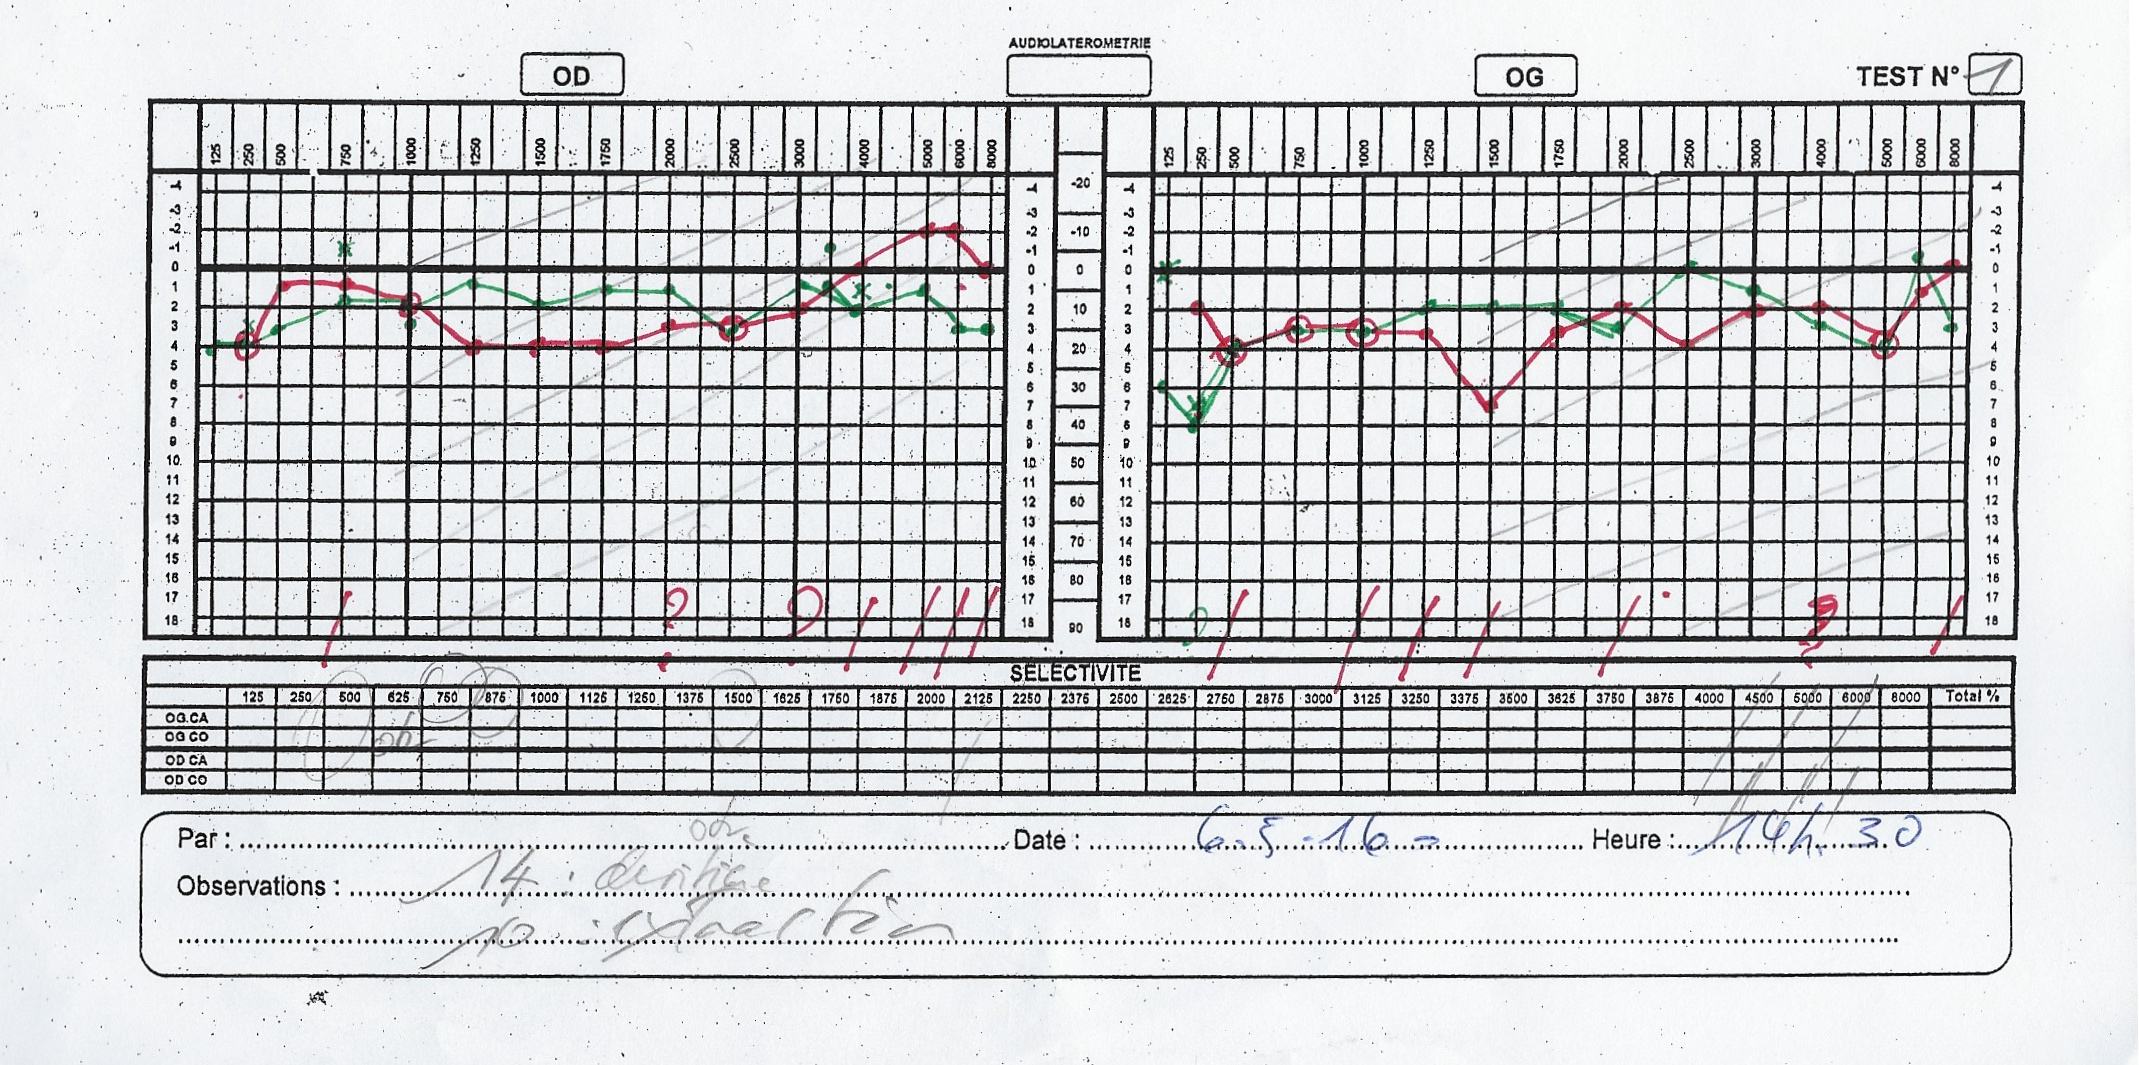
\includegraphics[scale=0.1,bb = 0 0 200 100, draft, type=eps]{PatientV1.jpg}}}
%}
\end{figure}
\end{quotation}

\chapter{Etude avec utilisation du test Tomatis en clinique psychiatrique.}

\section{Les tests d'écoute Tomatis : }

\paragraph{Hypothèse :}

\paragraph{Est-ce possible d'évaluer un travail musicothérapeutique au moyen
d'un test d'écoute?}

Est-ce que le processus d'écoute en musicothérapie améliore la capacité
d'écoute ?

Est-ce que les test auditifs avant et après la musicothérapie permettent
de visualiser l'action de la musicothérapie?

\paragraph{Y-a-t-il une modification de l'écoute du patient après une prise
en charge en musicothérapie ?}

\paragraph{Est-ce que les résultats( = un changement dans l'écoute) d'une prise
en charge musicothérapeutique peuvent être lisibles et visibles dans
un test d'écoute Tomatis ?}

Est-ce que ces résultats sont significatifs? 

\paragraph{Est-ce que l'écoute du patient s'est modifié ? si on a pu observer
une modification, dans quel sens va -t-elle ?}

Est-ce ce test valable ? est-ce que le contexte est suffisant pour
ressortir des résultats ?

\paragraph{Comment ?Nous allons vérifier, tester et comparer.}

\subparagraph{Un test d'écoute est une traduction graphique de l'écoute avec }

les paramètres suivants : 
\begin{itemize}
\item le son : dB, le volume de -20 à 90 et les Herz, fréquences de 125
à 8000. cf.ch.6.2.
\end{itemize}

\subparagraph{Par observation des courbes d'écoute relevées avec modèle de la courbe
idéale : équilibre, déséquilibre, harmonie, dysharmonie.}
\begin{itemize}
\item une interprétation psychologique va en être déduite, une constatation
de la posture d'écoute
\item une modification et une évolution ou transformation des courbes
\end{itemize}

\paragraph{Nous avons utilisé et fait en parallèle le test WHOQO-Bref avant
et après pour avoir une variable supplémentaire pour confirmer en
parallèle supposée de l'action de la musicothérapie.}

C'est une version test de 1997 issue Programme sur la santé mentale,
Organisation mondiale de la santé, Genève. Il y a 26 questions, que
le patient remplit lui-même en présence du thérapeute. p

Nous spécifions qu' il n'y a pas eu de traitement Tomatis et que le
suivi a été fait en musicothérapie sans exclure celui fait avec les
médecins, les psychologues, 

et les divers ateliers de créativité proposés dans cette clinique.

Nous avons pu organiser les tests d'écoute pour deux groupes : un
groupe en musicothérapie et un groupe de contrôle.
\begin{itemize}
\item 10 patients testés, groupe en musicothérapie : avant leur prise en
charge en musicothérapie; 2\textdegree{} test : après 4 semaines de
clinique. 
\item 9 patients testés, groupe de contrôle qui est un groupe sans musicothérapie
avec le même contexte, c.à.dire la clinique. 1\textdegree Test avant
le début des autres thérapies puis 2\textdegree{} test, après 4 semaines
qui équivalent à un séjour moyen en clinique, avant leur sortie.
\end{itemize}
Nous avons effectué les deux tests pour les deux groupes, avant et
après et fait remplir le questionnaire WHOQO-Bref.

A l'autre musicothérapeute, Regula Lehmann, travaillant régulièrement
à la clinique \footnote{Regula Lehmann, musicothérapeute à la clinique de Meiringen}
incombait la prise en charge complète de toutes séances en musicothérapie.

Nous mentionnons que ce sont des patients diagnostiqués avec une pathologie
de dépression, de burn-out et un cas de dépendance. 

Nous précisons que nous nous tiendrons à un comparatif de l'évolution
ou de la transformation de l'écoute, mais non de celles selon les
pathologies.

( à compléter.....)!


\chapter{Hypothèse : Réflexions et interrogations}

\section{Evaluation du travail fait en musicothérapie : }

Apprendre à écouter, c'est un travail et des résultats peuvent être
visibles. Nous utilisons un outil qui est le son. Nous accompagnons
le patient d'un point A pour aller au point B : que s'est -il passé
dans son écoute? Nous pouvons apporter des résultats visibles et tangibles
d'une forme d'apprentissage de l'écoute, d'une transformation de la
perception.On se base sur un graphique résultant d'un test de reconnaissance
de sons qui permet de visualiser une transformation psychologique
de l'écoute. 
\begin{itemize}
\item Il y a des résultats : nous pouvons constater soit un changement,
un statisme, un apprentissage,ou un refus d'apprendre et de se transformer.
Ce sont des données qui peuvent servir à mieux comprendre le patient
et à l'accompagner dans son cheminement.
\item Des questions sous-jacentes peuvent émerger comme celles-ci :
\end{itemize}
\begin{enumerate}
\item Quelle est la part d' objectivité ? de subjectivité?
\item S'il n'y a pas de changement visible dans le test , quelles conclusions
peut-on en tirer ? le changement va-t-il toujours de pair avec le
patient? synchronisé ou différencié dans le temps?
\item Est-ce normatif? par cette démarche, il y a le risque de catégoriser
et de paralyser le patient dans son parcours. Mais, cela peut aussi
l'aider dans son travail, son évolution. Ces deux possibilités sont
intrinsèques à tous les tests.
\end{enumerate}
\begin{itemize}
\item Nous sommes confrontés de plus en plus à donner des rapports aux caisse-maladies.
S'il y a une constatation de changement, de progression, le résultat
n'enfermera pas le patient dans une catégorie psychologique, qui,
transmise à celles-ci, pourrait lui être négative pour la poursuite
de son cheminement professionnel, via la vie active. 
\item Est-ce que ce test pourrait être un outil pour les thérapeutes et
les patients ? 
\item Avoir un support réel, visible car graphique pourrait-il être d'une
quelconque utilité pour le patient et pour le thérapeute ?
\item Est-il possible, à partir de deux tests d'écoute, de tirer des hypothèses
sur l'impact du son, de la musicothérapie, du soin par le son, sur
un patient ?
\item Le patient reste au centre de nos préoccupations.
\item Serait-ce un moyen, une façon de démontrer par ce moyen simple (autre
que l'Irmfct) que représente le test d'écoute l'utilité de la musicothérapie
? et ainsi de permettre une plus large acceptation et diffusion de
ce type de thérapie dans plus de milieux hospitaliers ou autres ?
\end{itemize}

\section{La musicothérapie et la méthode Tomatis : }
\begin{thebibliography}{10}
\bibitem{key-1}''Biologie Humaine , Principes d'anatomie et de physiologie'',
Elaine N.Marieb, 8ème édition, Pearson Education.

\bibitem{key-2}d Auriol (1996), \emph{La clé des sons, }Ed.Erès

\bibitem{key-3}Jean-Claude Ameisen (2013), \emph{Sur les épaules
de Darwin, Les battements du temps. }Ed\emph{.}Les liens qui libèrent

\bibitem{key-7}Silvia Bencivelli (2009),\emph{ Pourquoi aime-t-on
la musique?Oreille, émotion,évolution. }Ed.Belin.pour la science.

\bibitem{key-4}Simone Dalla Bella, Movement to Health Laboratory,
Université de Montpellier,lors de la XIIème Rencontre Cerveau-Esprit:
``Les rythmes'', 22 mars 2012, Sion, SUVA.

\bibitem{key-4}Rolando Omar Benenzon (2007)\emph{. La musicothérapie,
La part oubliée de la personnalité. }De Boeck

\bibitem{key-5}Emanuel Bigand (2012) \emph{Conférence, Musicothérapie
et Identité sonore.}Dijon, 6 avril 2012,\emph{ La musique comme outil
de stimulation cognitive. }In Richelle, (2013)\emph{Le cerveau mélomane
. }Belin

\bibitem{key-6}Isabelle Haugmard (2010) \emph{ABC de la thérapie
par les sons. }Michel Granch

\bibitem{Viret}Jacques Viret (2007) \emph{B. A-BA de la musicothérapie,}.
Pardès

\bibitem{key-9}Denis le Bihan \emph{Le cerveau de cristal, ce que
nous révèle la neuro-imagerie} (2012) Odile Jacob, sciences.

\bibitem{key-10}Antonio Damasio (2010) \emph{L'autre moi-même, les
nouvelles cartes du cerveau, de la conscience et des émotions }. Odile
Jacob,sciences.

\bibitem{key-12}Joseph-Marie Verlinde (1998) \emph{L'expérience interdite
.}Saint-Paul

\bibitem{key-13}L'essentiel, Cerveau et psycho (2011) \emph{Le cerveau
mélomane. }Revue de psychologie

\bibitem{key-14-1}Alfred Tomatis (1987) \emph{L'oreille et la voix.
}R. Laffont

\bibitem{key-2-1}Alfred Tomatis\emph{ }(1983)\emph{Vers l'écoute
humaine, }2ème Ed.Tome 2, Collection Science de l'éducation

\bibitem{key-3-1}Alfred Tomatis (1977) \emph{L'oreille et la vie,}
Ed.Robert Laffont

\bibitem{key-4-1}Alfred Tomatis (1972) \emph{De la communication
intra-utérine au langage humain, la libération d'Oedipe,} 5ème Ed.,\emph{
}Collection Science de l'éducation

\bibitem{key-5-1}Alfred Tomatis ((1989) \emph{Neuf mois au paradis,
histoires de la vie prénatale,} Ed.Ergo Press

\bibitem{key-6-1}Alfred Tomatis (1988)\emph{Les troubles scolaires,}
Ed.ErgoPress

\bibitem{key-3}Dominique Sandre, Docteur en médecine, spécialiste
en pédiatrie, conférence du 6 avril 2012, Dijon, \emph{Environnement
sensoriel du bébé dans un contexte hospitalier.}

\bibitem{key-1}Daniel Barenboim (2008), pianiste et chef d'orchestre,
\emph{La musique éveille le temps}. Ed.Fayard

\bibitem{key-2}Jean-Yves Bosseur (2005), \emph{Du Son au Signe, Histoire
de la notation musicale. }Ed. Alternatives

\bibitem{key-1}Emission''Envoyé spécial'', conçue et animée par
Pierre Lane

\bibitem{key-1}Patrick Dumas de la Roque ``L'écoute, c'est la vie'',
éd. Jouvence, trois Fontaines 

\bibitem{key-7}Fern Nevjinsky,\emph{ Adolescence, musique, Rorschach,
}, publication de l'Université de Rouen n\textdegree 215, source internet
décembre 2016.

\bibitem{key-1}E.Gendlin,\emph{ Focusing,} (2010) Ed. Pocket Evolution 

\bibitem{key-2}Felicitas Sigrist, \emph{Burnout und Musiktherapie,
Grundlagen, Forschungsstand und Praxeologie, }Ed. Zeitpunkt Musik,
Reichert Verlag Wiesbaden 2016

\bibitem{key-3}Hans-Helmut Decker-Voigt, S\emph{chulen der Musiktherapie,
}Ernst Reinhardt Verlag München Basel
\end{thebibliography}

\end{document}
